




平面上の幾何ベクトルを考える。互いに平行でない2つの幾何ベクトル${\bf e}_1, {\bf e}_2$を
考えよう。この平面上の任意の幾何ベクトル${\bf a}$について, ${\bf a}$を対角線とし, 
なおかつ${\bf e}_1, {\bf e}_2$にそれぞれ平行な辺を持つ平行四辺形を考えることができる
(${\bf e}_1, {\bf e}_2, {\bf a}$のそれぞれの始点を一致させて考える。図\ref{fig:vector_1}参照)。
中学校の理科でやった, 平行四辺形を使った力の分解を思い出せばよい。
\begin{figure}
    \centering
    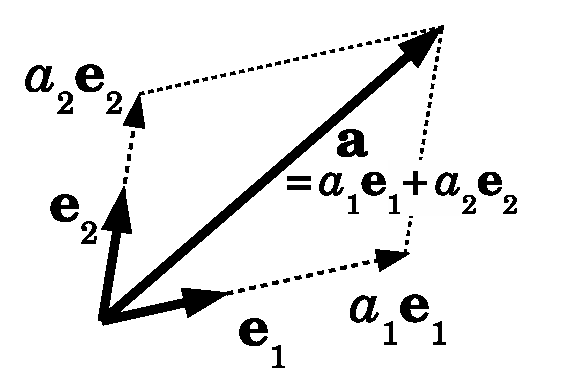
\includegraphics[width=5cm]{vector_1.eps}
    \caption{幾何ベクトル${\bf a}$を2つの幾何ベクトル${\bf e}_1, {\bf e}_2$
で分解する\label{fig:vector_1}}
\end{figure}

このとき, 図から明らかなように, ${\bf a}$は, 適当なスカラー$a_1, a_2$によって, 
\begin{eqnarray}{\bf a}=a_1{\bf e}_1+a_2{\bf e}_2\label{eq:vect_lincomb0}\end{eqnarray}
というふうに, ${\bf e}_1, {\bf e}_2$の線型結合で表すことができる。ここで 
線型結合の係数を並べると, 以下のような2次元数ベクトルができる(数を並べたものが数ベクトルだった!):
\begin{eqnarray}(a_1, a_2)\label{eq:vect_coordinate}\end{eqnarray}
逆に, 2次元の任意の数ベクトル$(a_1, a_2)$について, \eref{eq:vect_lincomb0}
のような幾何ベクトル${\bf a}$を考えることができる。
つまり, 「2つの幾何ベクトル${\bf e}_1, {\bf e}_2$の線型結合」という操作
を介して, 平面上の幾何ベクトルと2次元の数ベクトルが一対一に対応するのだ。

そこで, 幾何ベクトルを表す手段として, \eref{eq:vect_coordinate}のような数ベクトル
を使おう。それを「座標」という。すなわち, \eref{eq:vect_coordinate}で表される
数ベクトルを, \eref{eq:vect_lincomb0}で表される幾何ベクトル${\bf a}$の
\underline{座標} \index{ざひょう@座標} (coordinate)と呼ぶ。その数ベクトルの成分
($a_1$と$a_2$のそれぞれ)を「座標成分」と呼ぶ。そして, \textgt{これらの幾何ベクトルと
数ベクトルを同じものとみなしてしまう}。すなわち, 
\begin{eqnarray}
{\bf a}=a_1{\bf e}_1+a_2{\bf e}_2=(a_1, a_2)\label{eq:vect_alg_num}
\end{eqnarray}
と書いてしまうのだ。例えば, 
\begin{eqnarray}
{\bf a}=(2, 3)
\end{eqnarray}
と書かれる場合, これは, 一見, 数ベクトルだが, 
\begin{eqnarray}
{\bf a}=2{\bf e}_1 + 3 {\bf e}_2
\end{eqnarray}
という幾何ベクトルも意味する。また, 
\begin{eqnarray*}
{\bf e}_1=1{\bf e}_1+0{\bf e}_2\\
{\bf e}_2=0{\bf e}_1+1{\bf e}_2
\end{eqnarray*}
なので, ${\bf e}_1, {\bf e}_2$をそれぞれ座標で表すと次式になる:
\begin{eqnarray}
{\bf e}_1=(1, 0)\\
{\bf e}_2=(0, 1)
\end{eqnarray}

本来は幾何ベクトルを表すには矢印を描かねばならないし, そのスカラー倍や
足し算は作図で表さねばならないので面倒だが, 座標にしてしまえば, それは
数ベクトル, つまり数を並べたものなので, 書き表しやすいし, スカラー倍や足し算
も簡単である。

でも, ここで心配なことが出てくる: 幾何ベクトルのスカラー倍や足し算と, 
数ベクトルのスカラー倍や足し算とは, 本来, 全く別物である。従って, 幾何ベクトルを
座標で表して数ベクトルのルールで足し算したりスカラー倍したとしても, 
その結果が, 幾何ベクトルの足し算やスカラー倍の結果とつじつまあうのだろうか\footnote{もし, 
そのつじつまが合わないのならば, 幾何ベクトルを数ベクトルで表したときに, どこかで
不都合が生じてしまうだろう。}? それを確かめよう。\hv

\begin{q}\label{q:vect_add_2D} 平面内の2つの幾何ベクトル${\bf a}, {\bf b}$
が, それぞれ$(a_1,a_2)$と$(b_1,b_2)$というふうに座標で表されるとき, 
\begin{eqnarray}\alpha {\bf a}+\beta {\bf b}\end{eqnarray}
の座標は, 
\begin{eqnarray}\alpha (a_1,a_2) + \beta (b_1,b_2)\end{eqnarray}
と一致することを示せ($\alpha, \beta$は任意のスカラー)。ヒント:上の「座標成分」の定義
\eref{eq:vect_alg_num}に戻ること。
\end{q}\vspace{0.3cm}

ここで注意。${\bf e}_1$と${\bf e}_2$をどのように選択するか\footnote{大学数学では
${\bf e}_1, {\bf e}_2$の組み合わせを「基底」\index{きてい@基底}という。}によって, 
ひとつの幾何ベクトルについても様々な座標があり得る。従って, 幾何ベクトルと数ベクトル(つまり座標)
の対応関係の背後には, 常に「${\bf e}_1$と${\bf e}_2$をどのように選ぶか」が大きな問題
として存在している。

高校数学では, 簡単のため, ${\bf e}_1, {\bf e}_2$を, それぞれ大きさ(長さ)が1で, 互いに直交
するように選択する。そのような場合を, 大学数学では「正規直交座標系」という
\index{せいきちょっこうざひょう@正規直交座標系}\footnote{正規直交座標系を実現する
${\bf e}_1, {\bf e}_2$の組み合わせを「正規直交基底」という。} (図\ref{fig:vector_2})。
このとき, 「座標」とはすなわち, ${\bf a}$, ${\bf e}_1$, ${\bf e}_2$を同じ始点で描き, 
その始点を原点$O$とし, ${\bf e}_1$の向きを$x$軸, 
${\bf e}_2$の向きを$y$軸とするような$xy$座標を想定したとき, ${\bf a}$の終点の位置を
いわゆる$xy$平面の座標で表すことと同じである。

\begin{figure}
    \centering
    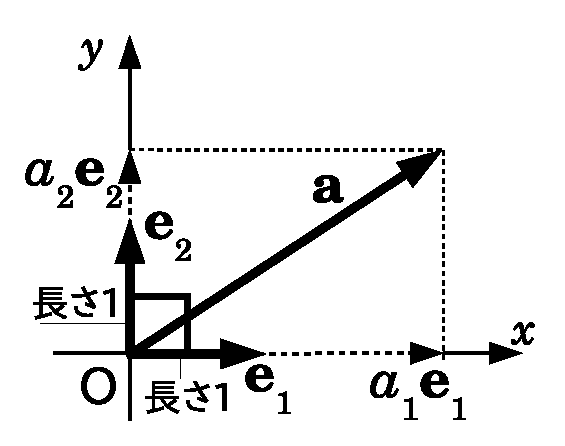
\includegraphics[width=5cm]{vector_2.eps}
    \caption{正規直交座標系。図\ref{fig:vector_1}の${\bf e}_1, {\bf e}_2$が互いに直交し, それぞれ大きさが1の場合に相当する。\label{fig:vector_2}}
\end{figure}

以後, 本書では, 特に断らない限り, 幾何ベクトルの座標は, 正規直交座標系について
考える。また, 特に断らない限り, 幾何ベクトルと数ベクトルを区別しないで
ベクトルと呼ぶ。


さて, 先に述べたように, 大きさが0であるような幾何ベクトルや, 全ての座標成分が0である
ような数ベクトルのことを\underline{零ベクトル}と呼ぶ。零ベクトルは
${\bf 0}$と表す\footnote{高校数学では$\vec{0}$と表す。
大学数学では単に0と表すこともあるが, こう書くと, 見掛け上, 数字(スカラー)の
0と全く区別がつかないので, その場その場に応じて, 
0はスカラーの0なのか, 零ベクトルなのか, 適宜, 空気を読んで判断しなければならない。}。




3次元空間のベクトルも, スカラー倍, 足し算, 内積を2次元平面のベクトルと同様に定義する。
すると, 3次元空間のベクトルは適当な3つのベクトルの線型結合で表せる
ので, 3次元の数ベクトル, つまり座標で表すことができる。正規直交座標系を使えば, 互いに直交する
3つの単位ベクトル${\bf e}_1, {\bf e}_2, {\bf e}_3$を使って, 任意のベクトル
${\bf a}, {\bf b}$は
\begin{eqnarray}
&{\bf a}=a_1{\bf e}_1+a_2{\bf e}_2+a_3{\bf e}_3=&(a_1, a_2, a_3)\\
&{\bf b}=b_1{\bf e}_1+b_2{\bf e}_2+b_3{\bf e}_3=&(b_1, b_2, b_3)
\end{eqnarray}
と書ける。このとき, 「線型結合」「内積」「長さ」は, 
\begin{eqnarray*}
&&\alpha{\bf a}+\beta{\bf b}=(\alpha a_1+\beta b_1, \alpha a_2+\beta b_2, \alpha a_3+\beta b_3)\\
&&{\bf a}\bullet{\bf b}=|{\bf a}||{\bf b}|\cos\theta =a_1b_1+a_2b_2+a_3b_3\\
&&|{\bf a}|= \sqrt{{\bf a}\bullet{\bf a}}=\sqrt{a_1^2+a_2^2+a_3^2}
\end{eqnarray*}
というように, 2次元平面と同様に座標で計算できる($\theta$は${\bf a}$と${\bf b}$のなす角)。
以下, 正規直交座標系で考える。
\mv






ところで, 物理学では, 何かの量を時刻$t$で微分することが多いので, 時刻$t$による微分を以下のような
特別な記号で表すことがよくある:
\begin{eqnarray}
x'(t)=\dot{x}\quad y'(t)=\dot{y}\quad {\bf r}'(t)=\dot{\bf r}
\end{eqnarray}
このように, 微分される関数の上に小さなドットをつけると, 「それを$t$で微分したもの」という意味になる。
\vv




\noindent{\textbf{答}}\ref{q:vect_linconv_def}
 複数のベクトルをそれぞれスカラー倍して足しあわせること。
\mv

% 平面内の2つの幾何ベクトル${\bf a}, {\bf b}$
\noindent{\textbf{答}}\ref{q:vect_add_2D} 
\eref{eq:vect_alg_num}より, ${\bf a}=a_1{\bf e}_1 + a_2{\bf e}_2$, 
${\bf b}=b_1{\bf e}_1 + b_2{\bf e}_2$だから, 
\begin{eqnarray*}
\alpha{\bf a}+\beta{\bf b}&=&\alpha(a_1{\bf e}_1 + a_2{\bf e}_2)+\beta(b_1{\bf e}_1 + b_2{\bf e}_2)\\
&=&(\alpha a_1 + \beta b_1){\bf e}_1 + (\alpha a_2 + \beta b_2) {\bf e}_2
\end{eqnarray*}
従って, $\alpha{\bf a}+\beta{\bf b}$の座標は, 
$(\alpha a_1 + \beta b_1, \alpha a_2 + \beta b_2)$
である。これは, $\alpha (a_1,a_2) + \beta (b_1,b_2)$に等しい。
\mv

% 上の問題で, $|{\bf a}|$と$|\bf b|$をそれぞれ求めよ
\noindent{\textbf{答}}\ref{q:vect_length_a_b} $|{\bf a}|=\sqrt{1^2+2^2}=\sqrt{5}$
\mv

\noindent{\textbf{答}}\ref{q:vect_inprod_coord2Drule} いま, ${\bf a}=(a_1, a_2)$, 
${\bf b}=(b_1, b_2)$とする。
\begin{enumerate}
\item ${\bf a}\bullet{\bf a}=(a_1, a_2)\bullet(a_1, a_2)=a_1^2+a_2^2$となる。
$a_1, a_2$は実数だから, $a_1^2\geq0$, $a_2^2\geq0$である。従って, $a_1^2+a_2^2\geq0$。
\item ${\bf a}\bullet{\bf a}=0$なら, $a_1^2+a_2^2=0$である。ところが, 前小問で
述べたように, $a_1^2\geq0$, $a_2^2\geq0$だから, これが成り立つのは$a_1^2=a_2^2=0$の
ときに限る。従って, $a_1=a_2=0$。従って${\bf a}=(0, 0)={\bf 0}$。
\end{enumerate}
(3)(4)(5)は略。
\mv

\noindent{\textbf{答}}\ref{q:vect_line2D4} $|2+2+1|/\sqrt{1^2+2^2}=\sqrt{5}$
\mv


% 空間ベクトル
% ${\bf a}=(1, 2, -1)$, ${\bf b}=(2, -1, -2)$として,
\noindent{\textbf{答}}\ref{q:vect_3D0} 
\begin{eqnarray*}
&&|{\bf a}|=\sqrt{1^2+2^2+(-1)^2}=\sqrt{6}\\
&&|{\bf b}|=\sqrt{2^2+(-1)^2+(-2)^2}=3\\
&&{\bf a}\bullet{\bf b}=1\times2+2\times(-1)+(-1)\times(-2)=2
\end{eqnarray*}
\mv




\section{指数関数}

「微分しても変わらない関数」, すなわち, 
\begin{eqnarray}
f'(x)=f(x)\label{eq:exp_start}
\end{eqnarray}
となるような関数$f(x)$は, どのような関数だろうか, 考えてみよう。
微分の定義(P.\pageref{sect_def_differential})を思い出せば, 
微小量(つまり十分に0に近い数) $dx$について, 
\begin{eqnarray}f(x+dx) = f(x) + f'(x) dx\end{eqnarray}
である。ここで$f'(x)=f(x)$であるということは, 
\begin{eqnarray}f(x+dx) = f(x) + f(x) dx\end{eqnarray}
ということである。これを変形すれば, 次式になる:
\begin{eqnarray}
f(x+dx)= (1+dx) f(x)
\end{eqnarray}

この式を, $x=0$や$x=dx$でそれぞれ考えれば, 
\begin{eqnarray}
&&f(dx)=f(0+dx)= (1+dx) f(0)\label{eq:expexplain3}\\
&&f(2dx)=f(dx+dx)= (1+dx) f(dx)\label{eq:expexplain4}\end{eqnarray}
である。\eref{eq:expexplain4}の右辺の$f(dx)$に\eref{eq:expexplain3}を入れれば, 
\begin{eqnarray}
f(2dx)= (1+dx)^2 f(0)\label{eq:expexplain42}
\end{eqnarray}
となる。同様に, $x=2dx$, $x=3dx$, ... などで考えれば, 1以上の任意の整数$N$について, 
\begin{eqnarray}
f(Ndx)= (1+dx)^N f(0)\label{eq:expexplain44}
\end{eqnarray}
となる。ここで$Ndx$をあらためて$x$とおけば, $N=x/dx$になるから, 
\begin{eqnarray}
f(x)&=& (1+dx)^{x/dx} f(0)\nonumber\\
    &=& \{(1+dx)^{1/dx}\}^x f(0)
\label{eq:expexplain6}
\end{eqnarray}
となる。この右辺の中の
\begin{eqnarray}
(1+dx)^{1/dx}\label{eq:Napier01}
\end{eqnarray}
に注目しよう。先に
言ってしまうと, 実は, これが第1章(\pref{eq:NapierNum_value})
に出てきたネイピア数$e=2.718\cdots$になるのだ。それを今から説明しよう。

$dx$は0に限りなく近い数である, ということをlimを使った式で書くと, \eref{eq:Napier01}は
\begin{eqnarray}
\lim_{h \to 0} (1+h)^{1/h}\label{eq:def_NapierNum_h}
\end{eqnarray}
となる。ここで$dx$を$h$と書き換えたのは, 他の本によく出てくる式の
形にあわせるため。なぜか数学ではlimで$0$に近づける変数を$h$と書くことが多い。

\begin{q}\label{q:exp_evalue} \eref{eq:def_NapierNum_h}のlimの内側を, 
$h=1/2$, $h=1/10$, $h=1/100$, $h=1/1000$, $h=1/10000$, $h=-1/10000$の
各場合について, 関数電卓で計算せよ。ヒント: 例えば$h=1/10$の場合は, 
$1.1^{10}$になる。1.1を10回掛けてもいいが, 
\pref{sec:calculator}を復習して関数電卓を上手に使おう。
\end{q}

この問でわかったように, やはり\eref{eq:def_NapierNum_h}は$2.718\cdots$に近づいていきそうだ。\\

\eref{eq:def_NapierNum_h}は別の形で表されることもよくある。$1/h$を$n$と書き換えよう。すると, 
$h$が0に近づく時, $n$は$\infty$に近づく($h>0$のときは)。そこで, \eref{eq:def_NapierNum_h}は
\begin{eqnarray}
\lim_{n \to \infty} \Bigl( 1 + \frac{1}{n} \Bigr)^n\label{eq:def_NapierNum}
\end{eqnarray}
とも書ける。問\ref{q:exp_evalue}の計算(最後のは除く)は, 
\eref{eq:def_NapierNum}のlimの内側について, $n=2$, $n=10$, 
$n=100$, $n=1000$, $n=10000$の場合にそれぞれ相当することは明らかだろう。

\eref{eq:def_NapierNum_h}, \eref{eq:def_NapierNum}が
\underline{ネイピア数}\index{ねいぴあすう@ネイピア数}$e$の定義である。

\begin{q}\label{q:def_NapierNum} \eref{eq:def_NapierNum_h}と\eref{eq:def_NapierNum}
をそれぞれ5回書いて記憶せよ。\end{q}

\begin{comment}
\begin{freqmiss}{\small\textgt{
ネイピア数$e$の定義は? と聞かれて, 「2.718, 以下, 
無限に値が続く数」と答えてしまう} ... それはダメ。$\pi$の定義も同様ですが, 
無理数は, どんなに多くの桁を答えても, それよりも多くの桁があり, その数字は
循環小数のようなパターンを持ちません。従って, 有限個の桁で数値を述べるのでは
無理数は定義できません。$e$の「正しい定義」は\eref{eq:def_NapierNum}。
この式は$e$に関する情報を全て含んでいます。これを使えば, 原理的には, 
何桁でも欲しいだけの精度で数値を計算することができます。}\end{freqmiss}
\end{comment}

\begin{freqmiss}{\small\textgt{\eref{eq:def_NapierNum}で, 
$n$を$\infty$ではなく0に近づける極限と勘違いして覚えてしまう} ... 
\eref{eq:def_NapierNum_h}の$h\rightarrow0$と\eref{eq:def_NapierNum}の
$n\rightarrow\infty$を混同しているのでしょうね。
仮に$n$を0.01や0.001などとして\eref{eq:def_NapierNum}を計算して
みましょう。2.718$\cdots$ではなく1に近づいて行ってしまいます。}\end{freqmiss}

というわけで, \eref{eq:expexplain6}の$\{\quad\}$の内側は, ネイピア数$e$
であることがわかった。すなわち, 「\textgt{微分しても変わらない関数}」は, 
\begin{eqnarray}
f(x)= e^x f(0)\label{eq:expexplain7}
\end{eqnarray}
である。特に, $f(0)=1$のときは, 
\begin{eqnarray}
f(x)=e^{x}
\end{eqnarray}
となる。この, $e$の累乗で表される関数, すなわち$e^x$のことを, 
\underline{エクスポーネンシャル} (exponential)\index{えくすぽーねんしゃる@エクスポーネンシャル} 
と呼ぶ。この関数は, 当然ながら微分しても変わらないはずだから, 
\begin{eqnarray}
(e^x)'=e^x\label{eq:exp_diff}
\end{eqnarray}
である。

\begin{faq}\small{\textgt{微分しても変わらない関数を
どうして考えようと数学者は思ったのですか?} ... どうしてでしょうね。
後で述べるように, これは実用的に重要なので, 
実用上の要請が発端かもしれませんね。}\end{faq}

\begin{faq}\small{\textgt{関数電卓って便利ですよね。買ったばかり
のころ説明書を読んで,こんなにも多くの機能があるのかと感動しました。}
... 数学を理解すれば関数電卓の威力は倍増します。}\end{faq}

エクスポーネンシャルを\underline{指数関数} \index{しすうかんすう@指数関数}と呼ぶこともある。
$e$以外の数を$x$乗した関数(例えば$2^x$とか)も「指数関数」と呼ばないわけではないが, 
一般には「指数関数」と言えば$e^x$のことをさすことが多い。なお, 第1章で述べたように, 
$e^x$を, $\exp x$\index{exp}と書くことも多い。単なる書き方の約束だが, 意外に見落とす
人がいるので, もういちど大きく書いておこう:

\begin{itembox}{約束}
\begin{eqnarray}\exp x :=e^x\end{eqnarray}
\end{itembox}

実は, $e^x$は, 次のようにも表される:
\begin{eqnarray}
e^x=\lim_{n \to \infty} \Bigl( 1 + \frac{x}{n} \Bigr)^n\label{eq:func_e_def}
\end{eqnarray}
なぜか? \eref{eq:func_e_def}の右辺で, $n/x=N$と置いてみよう。すると$n=Nx$なので, 
\eref{eq:func_e_def}の右辺は, 
\begin{eqnarray}
\lim_{n \to \infty} \Bigl( 1 + \frac{1}{N} \Bigr)^{Nx}\label{eq:func_e_def00}
\end{eqnarray}
となる。とりあえず$x>0$のときを考えると, $n\rightarrow\infty$のときは$N\rightarrow\infty$
であり, また, $Nx$乗を指数法則で書き換えると, 上の式は, 
\begin{eqnarray}
\lim_{N \to \infty} \Bigl[\Bigl( 1 + \frac{1}{N} \Bigr)^N\Bigr]^x\label{eq:func_e_def01}
\end{eqnarray}
となる。この[ ]内は\eref{eq:def_NapierNum}の形なので$e$である。従って, この式は$e^x$に
等しい, つまり\eref{eq:func_e_def}が成り立つ\footnote{$x\leq0$のときが気になる人へ: 
$x=0$のときは\eref{eq:func_e_def}の左辺も右辺も1なので成立。$x<0$のときは?
\eref{eq:func_e_def01}のlimが$N \to -\infty$に変わる。そのときも, 
\eref{eq:func_e_def01}は$e^x$である。なぜか? \eref{eq:def_NapierNum_h}
で$h<0$のときを考えると\eref{eq:def_NapierNum}が$n\rightarrow-\infty$でも
成り立つことがわかるだろう。}

これは\eref{eq:def_NapierNum}を拡張した形の式になっている。これは
統計学などでいずれ使う, 重要な式である。\hv


\begin{faq}{\small\textgt{問\ref{q:func_exp_interest1}(1)で, $1.01^{100}$を, 
\pref{eq:linear_approx02}でやった線型近似$(1+x)^a\fallingdotseq1+ax$
で計算したら, $1.01^{100}=(1+0.01)^{100}\fallingdotseq1+100\times0.01=1+1=2$
になってしまい, $2.7\cdots$にはなりません。何がおかしい?}
... 良いところに気づきました。その線型近似は, $a$が大きいと精度が悪いのです。}\end{faq}

\begin{faq}{\small\textgt{ネイピア数$e$というやつの不思議さに
驚きました。いったいどんな人が考えたんでしょうか?} ... 
ベルヌーイとかオイラーらしいです。ネイピアというスコットランド人(対数を
発明した人)の名前がついていますが, ネイピアが発見したのではないそうです。
ちなみにネイピア数の神秘は, さらにもっと続きがあるのです。}\end{faq}

さて, $y=e^x$のグラフはどうなるだろうか? どんな数も0乗は1だから, 
$e^0=1$である。従ってこのグラフは$(0, 1)$を通る。また, $x=1$のときは$y=e=2.718\cdots$だから, $(1, 2.718\cdots)$
を通る。$x$が1増えるたびに$y$は$2.718\cdots$倍になるので, $x$が大きくなるにつれて
このグラフは急速に上に伸びていくだろう。一方, $x=-1$のときは, 
$y=e^{-1}=1/e=1/2.718\cdots$となる。$x$が1小さくなるたびに$y$は$1/2.718\cdots$倍
になるので, $x$が負のほうに行くにつれて, グラフは急激に$x$軸に近づいて
来るだろう。そう考えると, $y=e^x$のグラフは図\ref{fig:y_expx}の実線のようになる。

君は, $e^x$が「微分しても変わらない関数」ということが, 
このグラフからなんとなく読み取れないだろうか? 微分(係数)は, グラフでは
接線の傾きだった。このグラフは, 右に行くほど, 値が大きくなるが, 傾きも
大きい。その大きくなるペースが(値と傾きで)ちょうど同じなのだ。
だから, $e^x$の微分は$e^x$になるのだ。

\begin{faq}{\small\textgt{うーん, その話, ちょっとよくわかりません} ... 
わからなければスルーでOK。数学はいろんな見方をすると理解が深まりますが, 
難しいときは1つの見方を理解するだけで構いません。先に進みましょう。}\end{faq}

図\ref{fig:y_expx}には, $y=e^{-x}$のグラフも示した。これは$y=e^x$のグラフを$y$軸に関して
対称移動したものだ(わからない人は\pref{sec:func_trans}の\ref{sec:func_trans}節を参照せよ)。\\
\begin{figure}[h]
    \centering
    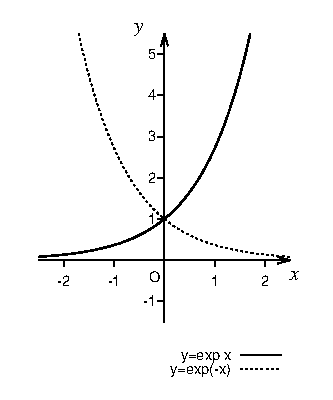
\includegraphics[width=6.0cm]{exp.eps}
    \caption{$y=\exp x$と$y=\exp(-x)$のグラフ}\label{fig:y_expx}
\end{figure}

エクスポーネンシャル以外の指数関数も, これらと似たグラフになる。例えば, 
$y=2^x$は, $y=e^x$よりはゆっくりだが, $x$の正の方向に行くにつれて
急激に増加する。








\section{三角関数の微分}

次に三角関数の微分を学ぼう。そのためには, まず, 微小量を三角関数に入れた時に
どうなるかを知らねばならない。ところが, \pref{eq:sinx_x}の\eref{eq:sinx_x}では既に, 
$\theta$が0に近ければ近いほど 
\begin{eqnarray}
\sin \theta \fallingdotseq \theta\label{eq:theta_sintheta}
\end{eqnarray}
であることを体験的に学んだ。これを証明しよう。
\begin{figure}[h]
    \centering
    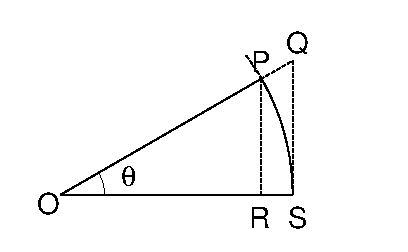
\includegraphics[width=6cm]{sinx_x.eps}
    \caption{単位円を切り取る扇形}\label{fig:sinx_x}
\end{figure}

\fref{fig:sinx_x}のように, 
単位円上で, 小さな角$\theta$によって切り取られる扇形OPSを考える。単位円の半径は1だから, 
OP=OS=1である。PからOSにおろした垂線の足をRとする。OPの延長線と, 点Sから真上に
伸ばした接線とが交わる点をQとする。円の半径(OS)と接線(QS)は直角だから, 角OSQは直角である。

図から明らかに, 弧PS$=\theta$, PR$=\sin \theta$, QS$=\tan \theta$である。

また, 面積を較べると, 
\begin{eqnarray}\bigtriangleup\text{OPS}<\text{扇形OPS}\end{eqnarray}
であることは図から明らかである。ところが, 
\begin{eqnarray}
&&\bigtriangleup\text{OPS}=\frac{\text{OS}\times\text{PR}}{2}=\frac{\sin\theta}{2}\\
&&\text{扇形OPS}=\frac{\text{弧PS}\times\text{OS}}{2}=\frac{\theta}{2}\label{eq:trigon_diff_5}
\end{eqnarray}
なので\footnote{扇形の面積は, 弧長×半径/2である。なぜか? 扇形の面積は, 弧長に比例することは直感的に
明らかだろう。従って, 半径$r$, 弧長$l$の扇形の面積は, 半径$r$の円の面積の$l/(2\pi r)$倍, つまり
$\pi r^2\times l/(2\pi r)=lr/2$となる。}, 
\begin{eqnarray}\frac{\sin\theta}{2}<\frac{\theta}{2}\end{eqnarray}
である。この両辺に2をかけて両辺を$\theta$で割れば, 
\begin{eqnarray}\frac{\sin\theta}{\theta}<1\label{eq:theta_sintheta1}\end{eqnarray}
である。また, 面積を較べると, 
\begin{eqnarray}\text{扇形OPS}<\bigtriangleup\text{OQS}\label{eq:trigon_diff_7}\end{eqnarray}
であることは図から明らかである。ところが, 
\begin{eqnarray}\bigtriangleup\text{OQS}=\frac{\text{OS}\times\text{QS}}{2}=\frac{\tan\theta}{2}\label{eq:trigon_diff_9}\end{eqnarray}
なので, \eref{eq:trigon_diff_5}, \eref{eq:trigon_diff_7}, \eref{eq:trigon_diff_9}より
\begin{eqnarray}\frac{\theta}{2}<\frac{\tan\theta}{2}\end{eqnarray}
である。この両辺に2をかけて, $\tan\theta=\sin\theta/\cos\theta$であることを思い出せば, 
\begin{eqnarray}\theta<\frac{\sin\theta}{\cos\theta}\end{eqnarray}
である。この両辺に$\cos\theta$をかけて両辺を$\theta$で割れば,
\begin{eqnarray}\cos\theta<\frac{\sin\theta}{\theta}\label{eq:theta_sintheta2}\end{eqnarray}
である。\eref{eq:theta_sintheta1}と\eref{eq:theta_sintheta2}より, 
\begin{eqnarray}\cos\theta<\frac{\sin\theta}{\theta}<1\label{eq:theta_sintheta3}\end{eqnarray}
である。ここで$\theta$が0に近づくと, $\cos\theta$は1に近づくので, \eref{eq:theta_sintheta3}の
左辺は1に近づく。そのとき, 1に近づく左辺と1(右辺)に挟まれて, 真ん中の$(\sin\theta)/\theta$も, 結局1に
近づく。従って, $\theta$が0に近ければ, 
\begin{eqnarray}\frac{\sin\theta}{\theta}\fallingdotseq 1\label{eq:theta_sintheta4}\end{eqnarray}
となり, \eref{eq:theta_sintheta}が成り立つ。特に, $\theta$を無限小$dx$で置き換えれば, 
$\fallingdotseq$は$=$になって, 次式が成り立つ:
\begin{eqnarray}
\sin dx = dx\label{eq:sindx}
\end{eqnarray}

この\eref{eq:sindx}が, 三角関数の微分への扉を開く鍵である。

まず, $\sin x$の導関数を調べよう。微分係数の定義
(\pref{eq:define_dif}の\eref{eq:define_dif})より, 
\begin{eqnarray}
\sin(x+dx) = \sin x + (\sin x)' dx\label{eq:deriv_sin03}
\end{eqnarray}
である。この左辺は, 加法定理と\eref{eq:sindx}より, 
\begin{eqnarray}
\sin(x+dx) = \sin x\, \cos dx + \cos x\, \sin dx\nonumber\\
= \sin x\, \cos dx + \cos x\,dx\label{eq:deriv_sin04}
\end{eqnarray}
となる。\eref{eq:deriv_sin03}, \eref{eq:deriv_sin04}より, 
\begin{eqnarray}
\sin x + (\sin x)' dx = \sin x\, \cos dx + \cos x\, dx\label{eq:deriv_sin05}
\end{eqnarray}
となる。$dx$は任意の微小量なので, \eref{eq:deriv_sin05}で$dx$を$-dx$
にしても成り立つはず($-dx$も微小量だから):
\begin{eqnarray*}
\sin x + (\sin x)'(-dx) = \sin x\, \cos(-dx) + \cos x\,(-dx)
\end{eqnarray*}
ここで, $\cos$は偶関数なので$\cos(-dx)=\cos dx$とし, ついでに多少整理すると, 
\begin{eqnarray}
\sin x - (\sin x)' dx = \sin x\, \cos dx - \cos x\, dx\label{eq:deriv_sin06}
\end{eqnarray}
となる。\eref{eq:deriv_sin05}から\eref{eq:deriv_sin06}を辺々引くと, 
\begin{eqnarray}
2(\sin x)' dx=2\cos x\,dx\label{eq:deriv_sin07}
\end{eqnarray}
となる。両辺を$2dx$で割って, 
\begin{eqnarray}
(\sin x)'=\cos x\label{eq:diffsin}
\end{eqnarray}
となる。すなわち, $\sin x$の導関数は$\cos x$なのだ!\mv

次に, $\cos x$の導関数を調べよう。まず, \eref{eq:trig_sinx_2pi}より, 
$\cos x=\sin(\pi/2 - x)$。これと\eref{eq:diffsin}より, 
\begin{eqnarray}
(\cos x)'&=&\Bigl\{\sin\Bigl(\frac{\pi}{2} - x\Bigr)\Bigr\}'
         =\cos\Bigl(\frac{\pi}{2} - x\Bigr)\,\Bigl(\frac{\pi}{2} - x\Bigr)'\nonumber\\
         &=&-\cos\Bigl(\frac{\pi}{2} - x\Bigr)
\end{eqnarray}
となる(ここで合成関数の微分公式を使った)。これは, \eref{eq:trig_cosx_2pi}より, $-\sin x$となる。
従って, 
\begin{eqnarray}
(\cos x)'=-\sin x\label{eq:diffcos}
\end{eqnarray}
となる。すなわち, $\cos x$の導関数は$-\sin x$である。\mv

では$\tan x$の導関数は? $\tan x=\sin x/\cos x$に\pref{eq:difdiv}の\eref{eq:difdiv}をあてはめればよい。
すなわち, $v=\sin x$, $u=\cos x$として, 
\begin{eqnarray}
(\tan x)'&=&\Bigl(\frac{v}{u}\Bigr)'=\frac{v'u-vu'}{u^2}\nonumber\\
&=&\frac{(\sin x)'\,\cos x-\sin x\,(\cos x)'}{\cos^2x}\nonumber\\
&=&\frac{\cos x\,\cos x-\sin x\,(-\sin x)}{\cos^2x}\nonumber\\
&=&\frac{\cos^2 x+\sin^2 x}{\cos^2x}=\frac{1}{\cos^2 x}\label{eq:difftan}
\end{eqnarray}
となる。以上をまとめると, 
\begin{eqnarray}
(\sin x)'&=&\cos x\label{eq:diff_sinx}\\
(\cos x)'&=&-\sin x\label{eq:diff_cosx}\\
(\tan x)'&=&\frac{1}{\cos^2 x}\label{eq:diff_tanx}
\end{eqnarray}
である。この3つの公式は必ず記憶しよう。




さて, 数値積分の問題をもうひとつやっておこう。この結果は, 後に統計学で使う。

\begin{q}\label{q:comp_int4} ガウス関数$f(x)=\exp (-x^2)$を考える。
\begin{enumerate}
\item 表計算ソフトで, $y=f(x)$のグラフを, $-4\leq x\leq 4$の範囲で描け。
ヒント: セルに数式を記述するとき, $-x^2$を「-x^2」のように表現するとうまく
いかない。表計算ソフトは, この記述を$(-x)^2$と解釈してしまうのだ。かわりに, 
「-x*x」とか, 「-(x^2)」と表現するとよい。
\item $f(x)$を$x=-4$から定積分してできる関数:
\begin{eqnarray}F(X)=\int_{-4}^{X}\exp(-x^2)dx\end{eqnarray}
を, $-4 \le X \le 4$の範囲で, 表計算ソフトを使って数値積分によって求め, 
その結果をグラフに描け。刻み幅は0.1程度でよい。
\item $F(4)$の値を述べよ。その値を$\sqrt{\pi}$の値と比較せよ。
\end{enumerate}
ここでは証明しないが, 以下のようになることがわかっている:
\begin{equation}\int_{-\infty}^{\infty} \exp(-x^2) dx=\sqrt{\pi}
\label{eq:integ_Gauss_func}\end{equation}
これを\underline{ガウス積分}\index{がうすせきぶん@ガウス積分}という。
\end{q}
\vv



さて, 加速度$a$は, P.\pageref{eq:Newton_eqmotion}の\eref{eq:Newton_eqmotion}で述べた, 
ニュートンの運動方程式
\begin{eqnarray}{\bf F}=m{\bf a}\label{eq:F_ma3}\end{eqnarray}
で定まる。ここで, $m$は物体の質量, ${\bf F}$は物体に働く力, ${\bf a}$は
物体の加速度である。


従って, ($m$は一定として) もし
力$F$が一定なら加速度$a$も一定である(逆に, 加速度$a$が一定なら力$F$は
一定だとも言える)。つまり, \textgt{等加速度直線運動は, 物体に働く力が
一定のときに実現する運動である}。例えば, 地表付近では質量$m$の物体には, 
\begin{eqnarray}F=mg\label{eq:Fgravity}\end{eqnarray}
という力が鉛直下向きに働く。ここで$g$は「重力加速度」と呼ばれる定数(厳密には, 
場所や標高によって多少変化する)であり, $g\fallingdotseq9.8\text{ m s}^{-2}$
である。\eref{eq:F_ma3}に\eref{eq:Fgravity}を代入すると, 
\begin{eqnarray}a=g\end{eqnarray}
となる。つまり, 地表付近の物体に重力だけが働いている時は, 大きさ$g$がほぼ
一定の加速度で物体は運動する(それが$g$を「重力加速度」と呼ぶ理由である)。

\begin{q}\label{q:int_velac} 地表付近で, 鉛直上向きに$x$軸を設定し, 時刻$t=0$のとき, $x=0$から鉛直上向き
に初速度$v(0)$でボールを投げ上げる。
\begin{enumerate}
\item 時刻$t$でのボールの位置$x(t)$と速度$v(t)$を, $t$, $v(0)$, $g$の式で表せ。
\item ボールの最高到達高度を$v(0)$と$g$の式で表せ。
\item ボールを高度100 mまで到達させるには, 初速度をどのくらい以上にしなければならないか?
\end{enumerate}\end{q}





\item 「$f$は, 複素数から複素数への写像である」
\begin{eqnarray}f: \mathbb{C} \rightarrow \mathbb{C}\end{eqnarray}
\item 「$f$は, 実数$x$を$x^2$に写す写像である」
\begin{eqnarray}x\in\mathbb{R}, f: x \mapsto x^2\end{eqnarray}



\begin{itemize}\item 今まで数学は受験に使う嫌なもの, 道具としてしかとらえていなかったけれど, 
これを機に, 数学の本当の楽しさ, 魅力が理解できるように努力したいと思います。\end{itemize}

がんばれー!





さて, 幾何ベクトルの内積(\eref{eq:def_inprod_00})と, 数ベクトルの内積(\eref{eq:def_inprod_01})
は, 少なくともここまでの段階では, 全く違うスタイルで定義されている。ところが, 座標の考え方をうまく使うと, 
これらが「同じもの」になってしまうのだ: いま, 平面上の2つの幾何ベクトルが, 正規直交座標系で
${\bf a}=(a_1, a_2)$, ${\bf b}=(b_1, b_2)$という座標で表されているとする。
\peref{eq:vect_alg_num}を思い出せば, これらは, 
\begin{eqnarray}
{\bf a}=a_1{\bf e}_1+a_2{\bf e}_2\\
{\bf b}=b_1{\bf e}_1+b_2{\bf e}_2
\end{eqnarray}
ということである。従って, これらの「幾何ベクトルの内積」は, 
\begin{eqnarray}
{\bf a}\bullet{\bf b}&=&(a_1{\bf e}_1+a_2{\bf e}_2)\bullet(b_1{\bf e}_1+b_2{\bf e}_2)\nonumber\\
&=&(a_1{\bf e}_1)\bullet(b_1{\bf e}_1)+(a_2{\bf e}_2)\bullet(b_1{\bf e}_1)\nonumber\\
&+&(a_1{\bf e}_1)\bullet(b_2{\bf e}_2)+(a_2{\bf e}_2)\bullet(b_2{\bf e}_2)\nonumber\\
&=&a_1b_1({\bf e}_1\bullet{\bf e}_1)+a_2b_1({\bf e}_2\bullet{\bf e}_1)\nonumber\\
&+&a_1b_2({\bf e}_1\bullet{\bf e}_2)+a_2b_2({\bf e}_2\bullet{\bf e}_2)\nonumber\\
&=&a_1b_1+a_2b_2\label{eq:vect_geom_coord_product}
\end{eqnarray}
となる。ここで, 内積の性質の(3), (4), (5)と, 
\begin{eqnarray}
&&{\bf e}_1\bullet{\bf e}_1={\bf e}_2\bullet{\bf e}_2=1\\
&&{\bf e}_1\bullet{\bf e}_2=0
\end{eqnarray}
である(つまり${\bf e}_1$, ${\bf e}_2$はともに単位ベクトルで, 互いに直交している)ことを使った。
一方, ${\bf a}, {\bf b}$を数ベクトルとみて「数ベクトルの内積」つまり\eref{eq:def_inprod_01}
を求めると, 
\begin{eqnarray}
{\bf a}\bullet{\bf b}=(a_1, a_2)\bullet(b_1, b_2)=a_1b_1 + a_2b_2\label{eq:inprod_coord0}
\end{eqnarray}
となる。なんと驚くべきことに, \eref{eq:vect_geom_coord_product}と\eref{eq:inprod_coord0}
が一致しているではないか! つまり, 正規直交座標系を採用する限り, 幾何ベクトルの内積は, 
数ベクトルの内積と一致するのだ。







\begin{q}\label{q:univ_lin_approx0} $x=0$付近で, 以下の式が成り立つことを示せ(ただし$a$は任意の実数)。
これらは全て重要な近似公式なので記憶せよ。
\begin{edaenumerate}
\item $\sin x \fallingdotseq x$
\item $\tan x \fallingdotseq x$
\item $\cos x \fallingdotseq 1$
\item $e^x \fallingdotseq 1+x$
\item $\ln (1+x) \fallingdotseq x$
\end{edaenumerate}\end{q}


\begin{exmpl} $\,\,\,\,\,f(x)=\sin x$ を線型近似する:\\
$f'(x)=\cos x$なので, $f(0)=0, f'(0)=1$. 従って$x=0$付近で
\begin{equation}\sin x\fallingdotseq f(0)+f'(0)x = x\end{equation}
(例おわり)\end{exmpl}
\mv

\item $\sin (\pi/10)$ (正確には$0.3090\cdots$となる)
\item $\sin 5^{\circ}$ (正確には$0.0871\cdots$となる)
\item $\tan 10^{\circ}$ (正確には$0.1763\cdots$となる)
\item $\sqrt{10}$ (正確には$3.1622\cdots$となる)
\item $\sqrt[3]{10}$ (正確には$2.1544\cdots$となる)





% 解答: 線型近似
\noindent{\textbf{答}}\ref{q:univ_lin_approx0}  \
\begin{enumerate}
\item $f(0)=1$, 
       $f'(x)=a(1+x)^{a-1}$, $f'(0)=a$。\\
       $\therefore f(x) \fallingdotseq 1+ax$
\item $f(0)=0$, 
       $f'(x)=\cos x$,
       $f'(0)=1$。\\
       $\therefore f(x) \fallingdotseq x$
\item $f(0)=0$, 
       $f'(x)=1/\cos^{2}{x}$, 
       $f'(0)=1$。\\
       $\therefore f(x) \fallingdotseq x$
\item $f(0)=1$, 
       $f'(x)=-\sin{x}$,
       $f'(0)=0$。
       $\therefore f(x) \fallingdotseq 1$
\item $f(0)=1$, 
       $f'(x)=e^{x}$, $f'(0)=1$。\\
       $\therefore f(x) \fallingdotseq 1+x$
\item $f(0)=\ln 1=0$, 
       $f'(x)=1/(1+x)$, \\$f'(0)=1$。
       $\therefore f(x) \fallingdotseq x$ 
\end{enumerate}
\hv

%
\noindent{\textbf{答}}\ref{q:univ_lin_approx2}  \
\begin{enumerate}
\item $f(0)=1$, 
       $f'(x)=1/(2\sqrt{1+x})$, $f'(0)=1/2$。
       $\therefore f(x)\fallingdotseq 1+x/2$。\\
別解:問\ref{q:univ_lin_approx0}(1)で$a=1/2$とすればよい。
\hv
\item $f(0)=1$, 
       $f'(x)=-1/(1+x)^2$, $f'(0)=-1$。
       $\therefore f(x)\fallingdotseq 1-x$。\\
別解:問\ref{q:univ_lin_approx0}(1)で$a=-1$とすればよい。
\hv
\item $f(0)=1$, 
       $f'(x)=1/(1-x)^2$, $f'(0)=1$。\\
       $\therefore f(x)\fallingdotseq 1+x$。\\
別解:前小問の結果で$x$を$-x$とすればよい。
\hv
\item  
\begin{eqnarray*}
&&f(0)=1,\,\, f'(x)=-\frac{1}{2}(1+x)^{-3/2},\,\, f'(0)=-\frac{1}{2}\\
&&\therefore f(x)\fallingdotseq 1-\frac{x}{2}
\end{eqnarray*}
別解:問\ref{q:univ_lin_approx0}(1)で$a=-1/2$とすればよい。
\end{enumerate}
\hv

% 
\noindent{\textbf{答}}\ref{q:univ_lin_approx4} 
\begin{enumerate}
\item $(0.99)^{10}=(1-0.01)^{10} \fallingdotseq 1-10 \times 0.01=0.9$
\item $\sin (\pi/10) \fallingdotseq \pi/10 \fallingdotseq 0.31$
\item $\sin 5^{\circ} = \sin \pi/36 \fallingdotseq \pi/36 \fallingdotseq 0.087$
\item $\tan 10^{\circ} =\tan \pi/18 \fallingdotseq 0.17$
\item 
\begin{eqnarray*}
&&\sqrt{10} =\sqrt{9+1} =3\sqrt{1+\frac{1}{9}} \fallingdotseq 3\Bigl(1+\frac{1}{2}\times\frac{1}{9}\Bigr)\\
&&=3\Bigl(\frac{19}{18}\Bigr)=\frac{19}{6} \fallingdotseq 3.17
\end{eqnarray*}
\item
\begin{eqnarray*}
&&\sqrt[3]{10}=10^{1/3}=(8+2)^{1/3}=\Bigl\{8\Bigl(1+\frac{2}{8}\Bigr)\Bigr\}^{1/3}\\
&&=2\Bigl(1+\frac{2}{8}\Bigr)^{1/3}=2\Bigl(1+\frac{1}{4}\Bigr)^{1/3}\\
&&\fallingdotseq 2\Bigl(1+\frac{1}{3}\times\frac{1}{4}\Bigr)=2\times \frac{13}{12}=\frac{13}{6}\fallingdotseq 2.17
\end{eqnarray*}
\end{enumerate}
\hv






\section{アレニウス型関数}\index{あれにうすがたかんすう@アレニウス型関数}

実は, 前節で学んだ「反応速度定数」$k$は, 温度によって決まる。温度が高いと
反応は進みやすいので$k$は大きな値になる。その様子は, 以下のような
関数で表すことができる(理由はここでは触れない):
\begin{eqnarray}
k=A\exp\Bigl(-\frac{E_a}{RT}\Bigr)\label{eq:k_Arrhenius}
\end{eqnarray}
ここで, $A$は正の定数で, 「頻度因子」と呼ばれる。$E_a$も正の
定数で, 「活性化エネルギー」と呼ばれる。これらはいずれも物質ごとに
異なる値をとる。$T$は絶対温度, $R$は気体定数と呼ばれる定数
(その値は8.31~J~mol$^{-1}$K$^{-1}$; 物質によらない)
である。\eref{eq:k_Arrhenius}を\underline{アレニウスの式}という
\footnote{\small 注: \eref{eq:diffeq0}という形の微分方程式が
\eref{eq:diffeq000_IC}という解(ここでは\eref{eq:chem_react7}がそれに
相当する)を持つのは, $a$(ここでは$-k$がそれに相当する)
が定数のときである。もし実験中に溶液の温度が時間と共に変わってしまうなら, 
$k$が時間とともに変わってしまうので, この条件が壊れる。つまり, 
実験中の温度が一定でないと, \eref{eq:chem_react7}と実験結果は
乖離する可能性がある。}。

\eref{eq:k_Arrhenius}のグラフは, ある$A$と$E_a$の値について, 
図\ref{fig:Arrhenius}(上)のようになる。このグラフの見方には
注意が必要である。まず, 横軸の"$T$/K"というラベルに
注目して欲しい。この斜字体の$T$は絶対温度, 立体Kはその単位であるKを表している。
SI単位系の決まりでは, 変数は斜字体, 単位は立体で表すことになっていたが, 
このグラフでは忠実にそれを守っている。また, "$T$~/~K"の/は割り算を意味する。
例えば$T=600$~Kなら, その両辺をKで割って, $T$~/~K=600である。このような
$T$~/~Kは無次元量であり, その値が横軸に書かれている。

縦軸も同様である。$k$は反応速度定数で, L~mol$^{-1}$~s$^{-1}$はその単位
である。従って, $k$~/~L~mol$^{-1}$~s$^{-1}$の値は無次元量となり, その
値が縦軸に書かれている。

このグラフから, 温度$T$の増加とともに$k$は急激に大きくなることがわかる。\\

\begin{figure}[h]
    \centering
    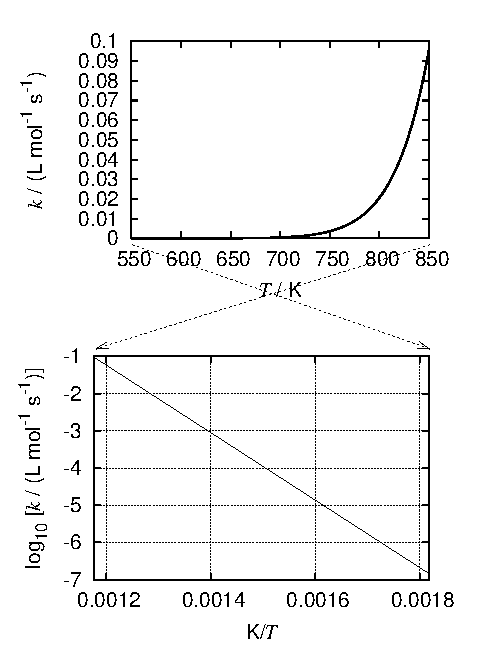
\includegraphics[width=8cm]{Arrhenius.eps}
    \caption{アレニウスの式のグラフ(例)。
% もとは$A=5.51\times10^9$ L/(mol s), $E_a=41.2$ kcal/molのとき。← 「化学I」プリントより。
上は, 素直に温度$T$を横軸に, 反応速度定数$k$を縦軸にプロットしたもの(普通のグラフ)。
下はアレニウスプロット。上のグラフの右の方(高温域)はアレニウスプロット(下のグラフでは)左の方に来る。同様に, 上の
グラフの左の方(低温域)はアレニウスプロットでは右の方に来ることに注意!}\label{fig:Arrhenius}
\end{figure}

次に, 図\ref{fig:Arrhenius}(下)のグラフを見て欲しい。これは, 上のグラフと
同じ関数, すなわち\eref{eq:k_Arrhenius}をプロットしたものだが, その表記法
において, 上のグラフとの違いが2つある。まず, 横軸を, 上のグラフの逆数, 
つまりK/$T$でとっている。例えば横軸の値が0.0014の
ときは, K/$T$=0.0014だから, この両辺に$T$をかけ, さらに両辺を0.0014で割ると, 
$T$=K/0.0014$\fallingdotseq$714~Kとなる。また, 縦軸は, 上のグラフの常用対数を
とったものである。例えば縦軸の値が$-2$のときは, 
$\log_{10}$[$k$~/~(L~mol$^{-1}$~s$^{-1}$)]=$-2$ということだから, 
$k$~/~(L~mol$^{-1}$~s$^{-1}$)=10$^{-2}$, すなわち
$k$=10$^{-2}$~L~mol$^{-1}$~s$^{-1}$ということだ。

図\ref{fig:Arrhenius}(下)のように, 
何かの量(ここでは反応速度定数)の量の対数を縦軸に, 「絶対温度の逆数」を横軸
にプロットするようなグラフを「アレニウスプロット」という。

さて, \eref{eq:k_Arrhenius}は, 図\ref{fig:Arrhenius}(下), すなわち
アレニウスプロットでは, 右下がりの直線になってしまった。なぜだろう?

\begin{q}\label{q:k_Arrhenius_log1} \eref{eq:k_Arrhenius}の両辺の常用対数をとることで, 次式を
導け:
\begin{eqnarray}
\log_{10}k&=&-\Bigl(\frac{E_a\log_{10}e}{R}\Bigr)\,\frac{1}{T}+\log_{10}A\label{eq:k_Arrhenius_log}
\end{eqnarray}\end{q}
\mv

ここで, $\log_{10}k$を$y$, $1/T$を$x$と置くと(それはアレニウスプロットを描く
のと同じ操作), \eref{eq:k_Arrhenius_log}は, 
\begin{eqnarray}
y=-\Bigl(\frac{E_a\log_{10}e}{R}\Bigr)\,x+\log_{10}A\label{eq:k_Arrhenius_log3}
\end{eqnarray}
という形の式, つまり$y$は$x$の一次関数になる。従って, アレニウスプロットではグラフは
直線になるのだ。このとき, 明らかに, 
\begin{eqnarray}
&&\text{傾き}=-\frac{E_a\log_{10}e}{R}\\
&&\text{切片}=\log_{10}A
\end{eqnarray}
である。従って, アレニウスプロットにおいて, 
\begin{eqnarray}
&&E_a=-\text{傾き}\times\frac{R}{\log_{10}e}=-\text{傾き}\times R\ln 10\label{eq:Arrhenius_E_a}\\
&&A=10^{\text{切片}}\label{eq:Arrhenius_A}
\end{eqnarray}
である($1/\log_{10}e=\ln 10$であることを使った)。グラフから傾きと切片を
読み取ってこの式に入れれば, $E_a$と$A$の値を求めることができる。


\begin{q}\label{q:k_Arrhenius_log3} 図\ref{fig:Arrhenius}(下)のグラフから
$E_a$と$A$の値を推定しよう。$x$は横軸の値, $y$は縦軸の値とする。
なお, 以下の読み取りは, 定規を使ってかなり慎重にやらないと, 良い結果は
得られない。
\begin{enumerate}
\item $x=0.0012$のときの, この直線上の$y$の値を読み取れ。
\item $x=0.0018$のときの, この直線上の$y$の値を読み取れ。
\item それらから, 直線の傾き(それを$a$と置く)を求めよ。
\item 直線の式を$y=ax+b$とし($a$は小問(3)で求めた), $x$, $y$に小問1の値を
代入することで, 切片$b$の値を求めよ。
\item $a$を\eref{eq:Arrhenius_E_a}に代入することで, $E_a$の値を求めよ(単位を忘れないように!)。
\item $b$を\eref{eq:Arrhenius_A}に代入することで, $A$の値を求めよ(単位を忘れないように!)。
\end{enumerate}
\end{q}

%ここで注意! アレニウスプロットでは, 横軸は「絶対温度の逆数」なので, その値が大きくなるという
%ことは, 絶対温度は小さくなる, ということである。つまり, アレニウスプロットでは, 右に行くほど
%低温の状況を表し, 左に行くほど高温の状況を表すのだ。

\begin{faq}{\small\textgt{さきほどの問で, アレニウスプロットの切片を$\beta$としましたが, 
それは$1/T$が0のときの$\log_{10} k$の値のことですよね。でも, $1/T=0$って, ありえなくない
ですか? 温度$T$を無限大にする? そんなこと, 実際にできます?} ... 実際の実験や観測では, 
「無限大の温度」など不可能ですし, 従って$1/T=0$となることはあり得ません。でも, グラフの
上では, アレニウスプロットの式はアレニウスプロットでは直線になりますので, それを左の
ほうにまっすぐ伸ばしていけば, いずれ端っこ($1/T=0$に対応する点)に至ります。そこでの
縦軸の値を読めばいいのです。こういう操作を「外挿」と言います。}\end{faq}

\begin{faq}{\small\textgt{アレニウスプロットではなぜ常用対数をとるのですか? アレニウスの
式には$e$が出てくるので, 自然対数のほうがすっきりしませんか?} ... 私もそう思いますし, 
実際, 自然対数でやれば, \eref{eq:k_Arrhenius_log}, \eref{eq:k_Arrhenius_log2}で
出てきたような$\log_{10}e$や$\ln 10=2.303...$などの数が出てこなくて, すっきりします。
常用対数でやるのは慣習です。昔, コンピュータが未発達のころは, データを実際に手で
片対数グラフ用紙に描き込んでいたので, 常用対数のほうがやりやすかったのでしょう。}\end{faq}

さて, 反応速度定数以外にも, 物理学・化学・生物学では, 様々な量が, 温度$T$に対して
\eref{eq:k_Arrhenius}の右辺のような形の関数で依存することが極めて多い。そこで
このような形の関数を「アレニウス型関数」\index{あれにうすがたかんすう@アレニウス型関数}
と呼ぶ。アレニウス型関数で表現される量なら, その温度依存性は, アレニウスプロット
では必ず直線になる。なので, 君はこれから, 様々な機会で, アレニウスプロットを目にすることだろう。\\


\noindent{\textbf{答}}\ref{q:k_Arrhenius_log1} 略。\\

\noindent{\textbf{答}}\ref{q:k_Arrhenius_log3} (1) 約$-1.21$。(2) 略。(3) 約$-9050$。\\
(4) 約9.65。(5) 約173000 J/mol。\\
(6) 4.5$\times10^9$~L~mol$^{-1}$~s$^{-1}$。
%ほんとは Ea=41500 kcal/mol = 173885 J/mol
%ほんとは A=4.5*10^9 L /mol /s
\vv












ところで, \eref{ed:def_Pa}で述べた「運動の法則 (ニュートンの運動方程式)」
は, 高校の教科書や参考書では, \\
「質量$m$~(kg)の物体が力$F$~(N)
を受けたとき, 物体の速度は変化する。その変化率, つまり加速度を
$a$~(m~s$^{-2}$)とすると, $F=ma$が成り立つ」\\
というふうに, $F, m, a$などに単位を添えて書くことがある。しかし
これは蛇足である。$F=ma$のような自然法則は, $F, m, a$をそれぞれ
どのような単位で表そうが成り立つのである。

\begin{exmpl}
$F=6$~N, $m=2$~kg, $a=$3~m s$^{-2}$のとき, $F=ma$が成り立つことは
明白だろう。ところがこれを, $F=6$~N, $m=2000$~g, $a=$300~cm s$^{-2}$
というふうに, 一部を別の単位で書き換えたら, $F=ma$は成り立つだろうか? 
右辺は$ma=2000$~g$\times$300~cm~s$^{-2}$~=600000~g~cm~s$^{-2}$
となる。ここで出てきた600000という数値は, $F=6$~Nの6とはあまりに
かけ離れているので, 一見すると, $F=ma$は成り立っていないようにも
見える。しかしそれは数値だけに注目しているからそう思うだけなのだ。
単位もちゃんと考えれば, $ma$= 600000~g~cm~s$^{-2}$ =600000($10^{-3}$~kg)($10^{-2}$~m)~s$^{-2}$
= 600000$\times10^{-5}$~kg~m~s$^{-2}$= 6~kg~m~s$^{-2}$ = 6 N=$F$なので, 
$F=ma$は成り立っているのである。(例おわり)\end{exmpl}

このように, それぞれの物理量をどのような単位であらわしても, 
計算途中で全ての単位をきちんと追いかけ, 必要に応じて変換
してやれば, 最後の結果は必ず辻褄が合うのだ。なので, 物理量
を変数で表すときに単位まで指定する必要は無いし, 無理に
指定すると, その式があたかも特定の単位でしか使えないもの
であるかのような, 誤った印象を与えてしまう。

それにもかかわらず, 上述のような蛇足が教科書等でなされるのは, 
最初に厳しく単位を限定しておけば, 単位換算に起因するミスの
多くを防げるからである。君も, \textgt{物理量はできるだけSI基本単位か, 
その組立単位で表現し, kgのk以外の接頭辞は10の何乗というふうに
置き換えてから, 式に代入するようにしよう}。\\

ちなみに, 世の中には, 特定の単位でしか使えないような式も存在
する。そのような場合は, 変数に単位を添え書きすることは蛇足ではなく, 
意味がある。そのような場合の多くは, 数値の計算を簡便にすることを
目的とした式や, 経験的な近似式である。\\

\begin{exmpl} 空気が含むことのできる水蒸気量は, 気温に依存する。
いま, 飽和水蒸気圧(その空気が最大限に水蒸気を含むときの, 水蒸気の
分圧)を$e$~(hPa)とし, 気温を$t$~(${}^\circ\mathrm{C}$)とすると, 
\begin{eqnarray}
e \fallingdotseq 6.1078\times10^{\frac{7.5 t}{t+237.3}}
\end{eqnarray}
である。これをティーテンスの式という。この式では, 
気温は必ず${}^\circ\mathrm{C}$で表してから代入しなければ
ならないし, 出てくる結果は, 必ずhPaという単位で解釈しなければ
ならない。(例おわり)\end{exmpl}

\begin{q}\label{q:notation_wrong} 以下の記述において蛇足あるいは不適切な点を指摘せよ:
\begin{enumerate}
\item 物体に力をかけて移動させるとき, 力(N)と距離(m)の積を, 仕事(J)という。
\item 1秒あたりに何m進むかを速さという。
\item 気体定数$R$を有効数字3桁で表すと, $R=8.31$~J/mol$\cdot$Kである。 
\item 質量mの物体が加速度aで運動するとき, その物体に働く力Fは, F=maという式を
満たす。例えば, m=2$kg$, a=3$ms^{-2}$のとき, F=6$N$である。
\end{enumerate}
\end{q}

\noindent{\textbf{答}}\ref{q:notation_wrong}
\begin{enumerate}
\item (N), (m), (J)は不要。
\item これは速さをm/sという特定の単位で表すことまで要求
しており, 速さの定義を逸脱している。速さの定義としては, 
「単位時間あたりに進む距離を速さという」で十分である。その方が, 
m/s以外の単位でも速さを表現できるのでうれしい。
\item 組立単位の分母の表記が紛らわしい。$R=8.31$~J~mol$^{-1}$K$^{-1}$と書くべき。
\item 変数(m, a, F)の立体表記を全て斜体にし, 単位($kg, m, s$)の斜体表記を
全て立体にすべき。数値と単位の間, 単位と単位の間にそれぞれスペースをあけるべき。
修正後: 質量$m$の物体が加速度$a$で運動するとき, その物体に働く力$F$は, $F=ma$という式を
満たす。例えば, $m=2$~kg, $a=3$~m~s$^{-2}$のとき, $F=6$ Nである。
\end{enumerate}




\begin{q}\label{q:unit_conv1}
米国ではガソリンの体積はgal (ガロン)という単位で表し, 距離はmil (マイル)
という単位で表す\footnote{米国の日常生活では, SI単位がほとんど
通用しない。米国の科学者は日常で使う単位と研究で使う単位を使い分けるのだ!}。
おおよそ, 1~gal=3.785 L, 1~mil=1.609 kmである。
\begin{enumerate}
\item ある車の燃費(単位体積のガソリンでどれだけの距離を走るか)は24 mil~gal$^{-1}$である。
その燃費をkm L$^{-1}$に換算せよ。
\item ある車の燃費は12 km~L$^{-1}$である。その燃費をmil gal$^{-1}$に換算せよ。
\end{enumerate}
必要なら, これらの計算に電卓を使ってもよい。
\end{q}
\mv

\noindent{\textbf{答}}\ref{q:unit_conv1} 
\begin{eqnarray*}
(1)\,\,\,\,&&24\text{ mil gal}^{-1}=24\,\frac{\text{mil}}{\text{gal}}=24\times\frac{1.609\text{~km}}{3.785\text{~L}}\\
&&=24\times\frac{1.609}{3.785}\text{~km~L}^{-1}=10.20\text{~km~L}^{-1}\\
(2)\,\,\,\,&&12 \text{~km~L}^{-1}=12\,\frac{\text{km}}{\text{L}}=12\times\frac{(1/1.609)\text{ mil}}{(1/3.785)\text{ gal}}\\
&&=12\times\frac{1/1.609}{1/3.785}\text{ mil gal}^{-1}\\
&&=12\times\frac{3.785}{1.609}\text{ mil gal}^{-1}=28.23\text{ mil gal}^{-1}
\end{eqnarray*}
\vspace{0.5cm}







\begin{q}\label{q:alg_num1}
正負の奇数の全てからなる集合:\\
$\{\cdots, -5, -3, -1, 1, 3, 5, \cdots\}$は, 
足し算・引き算・掛け算・割り算のそれぞれについて, 閉じているかどうか述べよ。
\end{q}

\noindent{\textbf{答}}\ref{q:alg_num1} 
掛け算については閉じている(奇数と奇数の積は奇数)。その他については閉じていない。例えば
$3+1=4$や$3-1=2$は奇数でない。従って足し算・引き算について閉じていない。例えば$5/3$はそもそも整数
でないから奇数でない。従って割り算について閉じていない。\\



\begin{q}\label{q:unit_missing} (発展) 四則演算の公理に基いて, 以下を証明せよ。
ただし, $p, q, r, s$は任意の整数とし, それらが分数の分母に来る時は0ではないとする。
\begin{eqnarray}
&&q\times\frac{1}{p}=\frac{q}{p}\\
&&\frac{1}{p}\times\frac{1}{r}=\frac{1}{pr}\\
&&\frac{q}{p}\times\frac{s}{r}=\frac{qs}{pr}\\
&&\frac{q}{p}\div\frac{s}{r}=\frac{q}{p}\times\frac{r}{s}
\end{eqnarray}
\end{q}




整数でない有理数は, 小数で表すこともできる。小学校で習ったように, 小数は, 例えば
\begin{eqnarray}
13.2754
\end{eqnarray}
のように, 整数部(この場合は13)と小数部(この場合は, 2754)を, 
ドット(それを小数点と呼ぶ)で隔てて並記する。小数部に
おいて, 小数点に近い方から数えて$n$番目の数値を
「小数第$n$位」とか「小数点以下第$n$位」と呼ぶ(小数点は
含まずに数えることに注意せよ)。上の例では, 小数第3位は5
であり, 小数点以下第3位も5である。\\

$0.12$のように有限桁の小数も, $12/100$とできるから有理数である\footnote{もちろんこれは
約分して$3/25$とできる。しかし, それはここではどうでもいいことである。約分できようが
できまいが, とにかく「整数割る整数」で表されれば有理数である。}。$0.3333\cdots$は
無限に続く小数だが(このように同じような数の並びが延々と続く小数を\underline{循環小数}
\index{じゅんかんしょうすう@循環小数}という), $1/3$と表現できるから, 有理数である。

\begin{q}\label{q:alg_junkan} 
以下の循環小数を分数に書き換えてみよう。
\begin{eqnarray}x=0.90909090909090\cdots\label{eq:junkan0}\end{eqnarray}
\begin{enumerate}
\item 次式が成り立つことを確認せよ。
\begin{eqnarray}100x=90.909090909090\cdots\label{eq:junkan1}\end{eqnarray}
\item $100x-x=90$となることを確認せよ。
\item $x=10/11$となることを示せ。
\item 同様にして, $y=1.234234234234\cdots$を分数に書き換えよ。
\end{enumerate}
\end{q}
\mv

% 循環小数を分数に書き換えてみよう。
\noindent{\textbf{答}}\ref{q:alg_junkan} (略解)
\begin{enumerate}
\item \eref{eq:junkan0}の両辺を100倍する。
\item \eref{eq:junkan1}から\eref{eq:junkan0}を
辺々引き算する。
\item (2)より$99x=90$。この両辺を99で割って約分すると, $x=10/11$。
\item $1000y=1234.234234234\cdots$だから, $1000y-y=1233$となる。従って, $999y=1233$。
従って, $y=1233/999=137/111$。
\end{enumerate}


実数も, 足し算・引き算・掛け算・割り算(0で割る以外)について閉じている。このことは
直感的に明らかだが, 実は証明は簡単ではない(知りたかったら数学類に行こう!)。

全ての実数からなる集合(実数全体の集合)を, 慣習的に$\mathbb{R}$と表す。定義から明らかに, 
有理数は実数の一種である\footnote{「有理数と無理数をあわせて実数と呼ぶ」と定義したから, 
有理数は実数の一種である。}。すなわち, 
\begin{eqnarray}\mathbb{Q}\subset\mathbb{R}\end{eqnarray}
である。

\begin{freqmiss}{\small\textgt{「$\mathbb{R}$という記号は実数を表す」と思っている} ... 
違います。$\mathbb{R}$は「実数」ではなく, 「全ての実数からなる集合」です。}\end{freqmiss}



\begin{faq}{\small\textgt{ルートのつく数はすべて無理数なのですか? (循環する$\sqrt{x}$は無い?)}
... $x$が, いずれかの自然数の2乗になっている数(1, 4, 9, 16, ...)ならば, 
$\sqrt{x}$は有理数(というか自然数)です。それ以外の自然数$x$については
$\sqrt{x}$は必ず無理数になることが証明可能です(興味があればチャレンジして
ください)。}\end{faq}


\begin{exmpl} $a=b+c$という等式($a, b, c$は実数)を, 君はためらわずに
$a-c=b$のように変形するだろう($c$の移項)\index{いこう@移項}。
でも, なぜそのようなことができるのだろうか?

まず, \eref{eq:axiom_num_sum_inv}によると, 
$-c$という数がある。この数を, 
\begin{eqnarray}
a=b+c
\end{eqnarray}
の両辺に足すと, 
\begin{eqnarray}
a+(-c)=(b+c)+(-c)
\end{eqnarray}
となる。この式は, \eref{eq:alg_def_minus}より, 
\begin{eqnarray}
a-c=(b+c)+(-c)\label{alg_ikou_proof1}
\end{eqnarray}
となる。この右辺に\eref{eq:axiom_num_sum_assoc}を適用すると, 
\begin{eqnarray}
=b+\{c+(-c)\}
\end{eqnarray}
となる。さらにこれに\eref{eq:axiom_num_sum_inv}を適用すると, 
\begin{eqnarray}
=b+0
\end{eqnarray}
となる。さらにこれに\eref{eq:axiom_num_zero}を適用すると, 
\begin{eqnarray}
=b\label{alg_ikou_proof8}
\end{eqnarray}
となる。\eref{alg_ikou_proof1}$\sim$\eref{alg_ikou_proof8}から, 
\begin{eqnarray}
a-c=b
\end{eqnarray}
が証明できた! (例おわり)\qed
\end{exmpl}

\begin{exmpl} どんな数にも, 0を掛けたら0になる。なぜか? 
これも「当たり前だから」ではなく, 上の公理から証明されるのだ: 
まず, \eref{eq:axiom_num_zero}で$a$を0とおくと, 
\begin{eqnarray}
0+0=0
\end{eqnarray}
である。この両辺に, 任意の実数$x$をかけると, 
\begin{eqnarray}
x\times(0+0)=x\times0
\end{eqnarray}
これを, 分配法則(\eref{eq:axiom_num_distr})で展開すると, 
\begin{eqnarray}
x\times0+x\times0=x\times0
\end{eqnarray}
右辺の第2項(第1項でもよいのだが)を左辺に移項すると, 
\begin{eqnarray}
x\times0=x\times0-x\times0=0
\end{eqnarray}
従って, 任意の実数$x$に0をかけたものは0になる。\qed
(例おわり)\end{exmpl}


整数どうしの掛け算, 特に, 「マイナスの数を掛ける」という概念は, ちょっと難しい。
自然数の場合は, 掛け算は「何回か足すこと」と定義された。しかし, 例えば
「2を3回足す」ということの意味は明白だが, 「2を$-3$回足す」ということの意味
はよくわからない。というか, 意味が無い。そこで, 「マイナスの掛け算」においては, 
「何回か足す」という素朴な掛け算の概念を放棄する。そのかわりに, 自然数の足し算や
掛け算において自明とみなされた\eref{eq:axiom_num_sum_exch}$\sim$\eref{eq:axiom_num_sum_inv}
が, \textgt{自然数だけでなく整数においても成り立つ}ように, 
うまいこと「マイナスの掛け算」を定義してやるのだ。今からそのやり方を
説明する。\\

いま$a, b$を整数として, $a\times b$を考える。

$a, b$がともに正の整数(自然数)のときは, 自然数どうしの
掛け算の定義をそのまま使い, $a\times b$は「$a$を$b$回足す」ということ
にすればよい。

$a$が負の整数で, $b$は正の整数(自然数)のとき: 負の整数どうしの足し算
が可能なので, このときも, $a\times b$は負の整数$a$を$b$回足す, 
ということにすればよい(例えば$-3\times2$は, $(-3)+(-3)=-6$である)。

この逆の場合, つまり$a$が正の整数(自然数)で$b$が負の整数の場合は, 
\eref{eq:axiom_num_mult_exch}を使って$a\times b=b\times a$と
変形すれば, 負の数$b$を$a$回足す, ということにできる。

$b=0$のとき: $a$をゼロ回足す, すなわち, 何も全く足さない, ということと
解釈して, $a\times 0=0$とすればよい。$a=0$のときも, 
\eref{eq:axiom_num_mult_exch}を使って$0\times b=b\times 0=0$と
できる。



\begin{q}\label{q:alg_ineq3} (発展) 任意の実数$a, b$について
次式が成り立つことを証明せよ(三角不等式):\index{さんかくふとうしき@三角不等式}
\begin{eqnarray}
|a+b|\leq|a|+|b|
\end{eqnarray}
%\begin{enumerate}
%\item $(|a|+|b|)^2=a^2+b^2+2|ab|$を示せ。
%\item $|a+b|^2=a^2+b^2+2ab$を示せ。
%\item $(|a|+|b|)^2-|a+b|^2=2(|ab|-ab)$を示せ。
%\item $0 \leq |ab|-ab$を示せ。
%\item 以上より, $|a+b|^2 \leq (|a|+|b|)^2$を示せ。
%\item $0 \leq |a+b|$, $0 \leq |a|+|b|$を示せ。
%\item 以上より, $|a+b| \leq |a|+|b|$を示せ。
%\end{enumerate}
\end{q}


一方, \textgt{掛け算や割り算は, 違う次元の量どうしでも意味を持つ}。
例えば長さを時間で割ることは意味のある操作である(それによって速さが求まる)。
それに伴って, 次元も積(掛け算)や商(割り算)ができる{\small (和や差はできない)}: 
ある量$x$が, 別の量$y$, $z$で, $x=yz$のように表されるとき, $x$の次元は$y$の次元と$z$の次元の積に等しい。
つまり[$x$]=[$yz$]=[$y$][$z$]である。\\

\begin{exmpl} 面積という量の次元を考えてみよう。
長方形の面積$A$と2辺の長さ$a$, $b$には$A=ab$という関係がある。無論, 
$[a]=[b]=\mathsf{L}$である。従って, 
\begin{eqnarray}[\text{長方形の面積}]=[A]=[ab]=[a][b]=\mathsf{L}^2\end{eqnarray}
である。どのような図形でも, 面積の大小を長方形と比べたりできるので, 
その図形の面積は長方形の面積と同じ次元を持つ。従って, 
\begin{eqnarray}[\text{面積}]=[\text{長方形の面積}]=\mathsf{L}^2\end{eqnarray}
である。(例おわり)
\end{exmpl}\mv

このように, 何かの量の次元を求めたい時は, その最もシンプルな例を代表的
に考え, その次元を求めればよい。あるいは, その量の定義に戻って考えるとよい。

\begin{exmpl} 速さという量の次元を考えてみよう。速さは距離/時間なので, 
\begin{eqnarray*}
\text{[速さ]}=\text{[距離/時間]}=\text{[距離]/[時間]}=\mathsf{L}/\mathsf{T}
\end{eqnarray*}
となる。最後の項は, 以下のいずれの記法でもOKである:
\begin{eqnarray*}
\mathsf{LT}^{-1}\,\,\,\,\,\,\,\,\frac{\mathsf{L}}{\mathsf{T}}
\end{eqnarray*}
(例おわり)\end{exmpl}

\begin{q}\label{q:alg_dim0}
 以下の量の次元を, $\mathsf{L}, \mathsf{M}, \mathsf{T}$の組合せで表わせ。
\begin{edaenumerate}<3>
\item 体積
\item 密度
\item 加速度
\end{edaenumerate}
(ヒント: 密度は質量÷体積)
\end{q}
\vspace{0.2cm}

\begin{freqmiss}{\small\textgt{密度を「質量÷面積」だと勘違いし, [密度]=$\mathsf{ML}^{-2}$
だと思ってしまう} ... それは「面密度」というものです。単に「密度」と言えば, 普通は「質量÷体積」
のことです。}
\end{freqmiss}
\mv

このように, 世の中の様々な量の次元は, $\mathsf{L}$, $\mathsf{M}$, $\mathsf{T}$
などの, いくつかの基本的な次元またはそれらの積や商で表現される。\\


無次元は「次元が無い」ことではあるが, むしろ「無次元」も次元のひとつ, 
と捉える方が何かと考えやすい。実際, 多くの場合, 無次元量も「具体的な量」
である。例えば, 東京スカイツリーの高さを君の身長で割った値の次元は無次元だが, 
それは「君を何人分, 縦に並べると東京スカイツリーの高さに匹敵するか」という
具体的な量である。具体的な量である以上, 何らかの次元を与えてやりたいので
「無次元」も次元のひとつとみなすのだ(0もひとつの数である, というのと
なんとなく似ている)。

次元が無次元である量を無次元量
\index{むじげんりょう@無次元量}とか無名数\index{むめいすう@無名数}という。
個数も無次元量である。例えば1個のリンゴの質量に3を掛けると, 
同じ質量のリンゴを3個あつめたセットの質量になる。ところが"3個"という
量に, もし次元があったら, それを質量にかけた結果は[質量]以外の
次元になってしまう。これではつじつまがあわない。従って個数は無次元量
である\footnote{小学校で「ミカンとリンゴは違うからミカン2個と
リンゴ3個は足せない」と習った。
しかし, 2個も3個も「無次元」という同じ次元ならば, 足せるじゃないか! 
実は, 小学校で習ったことが少し乱暴なのだ。リンゴもミカンも「果物」
という観点で見なおせば, その和は「果物が何個か?」という, 意味を持つのだ。}。\\

さて, どんな等式(方程式・恒等式)も, 「左辺=右辺」という形をとる。これは
左辺と右辺の大小関係の比較の結果, 引き分けを表すものである。同様に, 不等式も
大小関係の比較の結果である。従って, \textgt{等式や不等式の左辺と右辺で次元は必ず一致する}。
これは, 君が数学以外の分野で, 式や数値を変形したり記憶するとき, 
ミスのチェックに使える。これを\underline{dimension check}\index{dimension check}という。

\begin{q}\label{q:dim_sphereSV} \eref{eq:ball_surface}, \eref{eq:ball_volume}
をもとに, [$S$]=[面積], [$V$]=[体積]であることを示せ。
\end{q}

\noindent{\textbf{答}}\ref{q:alg_dim0} 
\begin{enumerate}
\item 例えば立方体の体積$V$は, 立方体の一辺の長さを$a$とすると, $V=a^3$である。
従って, $[$体積$]=[$立方体の体積$]=[a^3]=[a]^3=\mathsf{L}^3$
\item $[$密度$]$=[質量/体積]=$\mathsf{ML}^{-3}$
\item 加速度は, 速度の変化を時間で割ったものだから, [加速度]=[速度/時間]=$\mathsf{LT}^{-2}$となる
(注: 厳密に加速度を定義するには, 微分という数学が必要)。
\end{enumerate}
\mv

\noindent{\textbf{答}}\ref{q:dim_sphereSV} \eref{eq:ball_surface}, \eref{eq:ball_volume}より, 
\begin{eqnarray*}
&&[S]=[4\pi r^2]=[4\pi][r^2]=[r^2]=\mathsf{L}^2=[\text{面積}]\\
&&[V]=\Bigl[\frac{4}{3}\pi r^3\Bigr]=\Bigl[\frac{4}{3}\pi\Bigr][r^3]=[r^3]=\mathsf{L}^3=[\text{体積}]
\end{eqnarray*}
である(ここで, 4や$4/3$や$\pi$は無次元の数値であることに注意!)。\qed




すなわち, \eref{eq:ball_surface}, \eref{eq:ball_volume}のそれぞれ
の次元を考えれば, これらを取り違えるというミスは簡単に防ぐ
ことができるのだ。

ちなみに, \eref{eq:ball_surface}で$S$はsurfaceの頭文字, \eref{eq:ball_volume}で
$V$はvolumeの頭文字, そして$r$はradiusの頭文字に由来する。このように, 特定の量を
表す文字は, その量を意味する英単語の頭文字が慣習的に使われることが多い。それも
公式を覚えたり思い出したりするときの手がかりになる。だから, 英語が苦手な人は
数学でも苦労するのだ。\vv


さて, 単位と次元は別の概念である。端的にいえば, 
例\ref{exmpl_earth_radius_dim_unit}
で見たように, \textgt{ひとつの次元にもいろんな単位があり得る}。

\begin{exmpl}
「君の身長」という量を$A$としよう。$A$の次元は?という問には, [長さ]
あるいは$\mathsf{L}$と答えることができる。それは$A$を定義した
時点で既に決まっている。

一方, $A$の単位は? $A=160$ cmと表すならcm, 
$A=1.6$ mと表すならmがそれぞれの単位だが, それは$A$の定義
(君の身長)から導かれることではない。「どの単位が便利か」
という別の判断によるのだ。従って, この問は意味が無い。(例おわり)
\end{exmpl}

\begin{freqmiss}{\small\textgt{次元を聞かれているのに単位を答えたり, 
単位を聞かれているのに次元を答える} ... 次元と単位は互いに関係するものの, 
別の概念です}。\end{freqmiss}

\begin{freqmiss}{\small\textgt{次元と単位をイコールで結んでしまう。
例えば, $\mathsf{M}\mathsf{L}^{-3}=$kg m$^{-3}$と書く} ... 
これは間違い。何度も言いますが, 次元と単位は別物。
$\mathsf{M}\mathsf{L}^{-3}=$[kg m$^{-3}$]と書くなら合っています。}\end{freqmiss}

\begin{q}\label{q:diff_dim_unit} 次元と単位はどう違うか?\end{q}




このうち, molは個数の単位なので, その表す量は無次元である。無次元の量に
単位があるのもちょっと奇妙だが, これは1個を単位としていては数があまりに
大きくなるのが煩わしいから使われる。例えば12個を1ダースと呼ぶのと同じようなものだ。



ところで, 前述した「運動の法則(ニュートンの運動方程式)」では\\
「質量$m$の物体が力$F$を受けたとき, 物体の速度は変化する。
その変化率, つまり加速度を$a$とすると, $F=ma$が成り立つ」\\
と述べた。この中に, 単位は一切, 出て来なかったことに注意しよう。
ところが, 中学校や高校の教科書・参考書などでは, \\
「質量$m$ (kg)の物体が力$F$ (N)を受けたとき, 物体の速度は変化する。
その変化率, つまり加速度を$a$ (m~s$^{-2}$)とすると, $F=ma$
が成り立つ」\\
とのように, 単位を添えて書くことがある。これは蛇足である。
$F=ma$は, $F, m, a$をそれぞれどのような単位で表そうが, それら
の単位どうしで整合性がとれていれば成り立つからである。そもそも
単位は量を数値で表すために人為的・便宜的に導入されるものだが, 
自然の法則や, そこに出てくる量は, そのような人間の勝手な都合
とは無関係に存在するはずだ(自然の法則は人類がいようがいまいが, 
存在するはずだ)。従って, そのようなものは, 単位を使わずに記述
できるはずだ, と考えるのだ。なので, 普通, 法則の記述は単位とは
できるだけ切り離すのだ。

そのような蛇足が教科書等でなされるのは, あくまで教育的
な配慮からである。質量は(SI単位では)kgで表すもの, ということが
すぐに頭に浮かんでこない人のための「補助輪」のようなものである。\\

\begin{q}\label{q:notation_wrong} 以下の記述において不適切あるいは稚拙な点を指摘せよ:
\begin{enumerate}
\item 物体に力をかけて移動させるとき, 力(N)と距離(m)の積を, 仕事(J)という。
\item 1秒あたりに何m進むかを速さという。
\item 気体定数$R$を有効数字3桁で表すと, $R=8.31 $J/mol$\cdot$Kである。 
\item 質量mの物体が加速度aで運動するとき, その物体に働く力Fは, F=maという式を
満たす。例えば, m=2$kg$, a=3$ms^{-2}$のとき, F=6$N$である。
\end{enumerate}
\end{q}




\noindent{\textbf{答}}\ref{q:unit_NJPaW_matome1}
ニュートンの運動方程式によると, 質量$m$の物体が力$F$を
受けたとき, 物体の加速度を$a$とすると, $F=ma$が成り立つ。
従って, $[\text{力}]=[F]=[m][a]=\mathsf{MLT}^{-2}$。
また, 物体に力をかけて移動させるとき, 力と距離の積を, 
「仕事」という。従って, $[\text{仕事}]=[\text{力}]\times[\text{距離}]$
$=(\mathsf{MLT}^{-2})(\mathsf{L})=\mathsf{ML}^2\mathsf{T}^{-2}$。
また, 面にかかる力を面積で割ったものを圧力という。
従って, $[\text{圧力}]=[\text{力}]/[\text{面積}]=$
$(\mathsf{MLT}^{-2})/\mathsf{L^2}=\mathsf{ML}^{-1}\mathsf{T}^{-2}$。
また, ある時間内になされた仕事や, 出入りした熱や, 
エネルギーの増減量を, その時間で割ったものを, 仕事率又は熱効率という。
従って, $[\text{仕事率}]=[\text{仕事}]/[\text{時間}]$
$=\mathsf{ML}^2\mathsf{T}^{-2}/\mathsf{T}=\mathsf{ML}^2\mathsf{T}^{-3}$。\\

\noindent{\textbf{答}}\ref{q:kineticE_dim} $[K]=[(1/2)m\,v^2]=[m][v]^2$
$=\mathsf{M}(\mathsf{L}/\mathsf{T})^2=\mathsf{M}\mathsf{L}^2\mathsf{T}^{-2}=[\text{仕事}]$。\qed

\noindent{\textbf{答}}\ref{q:potentialE_dim} $[U]=[mgh]=[m][g][h]=$
$[\text{質量}][\text{加速度}][\text{高さ}]=\mathsf{M}(\mathsf{LT}^{-2})\mathsf{L}$
$=\mathsf{M}\mathsf{L}^2\mathsf{T}^{-2}=[\text{仕事}]$。\\



\noindent{\textbf{答}}\ref{q:unit_NJPaW2SIfnd} 
\begin{enumerate}
\item N=kg~m~s$^{-2}$
\item J=kg~m$^2$~s$^{-2}$
\item Pa=N~m$^{-2}$=kg~m$^{-1}$~s$^{-2}$
\item W=J~s$^{-1}$=kg~m$^2$~s$^{-3}$
\end{enumerate}
\mv




$x$に関する多項式$P(x)$が, 別の2つの多項式$Q(x), r(x)$で, 
\begin{eqnarray}P(x)=Q(x)r(x)\label{eq:poly_div0}\end{eqnarray}
と因数分解できるとしよう。これを書き換えれば, 
\begin{eqnarray}\frac{P(x)}{Q(x)}=r(x)\end{eqnarray}
である。あるいは, 
\begin{eqnarray}P(x)\div Q(x)=r(x)\end{eqnarray}
とも書ける。

\begin{exmpl}  $x^2+4x-5=(x-1)(x+5)$である。従って, 
\begin{eqnarray*}
(x^2+4x-5)\div(x-1)&=&\frac{x^2+4x-5}{x-1}\\
&=&\frac{(x-1)(x+5)}{x-1}=x+5
\end{eqnarray*}
(例おわり)\end{exmpl}
\hv

この例では, 分母と分子の$(x-1)$が約分できたので, 分母は消えて, 結果は$x+5$という多項式になった。
ところが, 多項式の割り算には, このようにすっきりとは約分できない(割り切れない)場合も存在する:
\hv

\begin{exmpl}  
\begin{eqnarray}
(x^2+4x+5)\div(x+3)=\frac{x^2+4x+5}{x+3}
\end{eqnarray}
この式は, これ以上, 約分できないから, 割り算の結果は多項式にならない(分母が残っている)。
しかし, これを次のように考えることができる:
\begin{eqnarray*}
x^2+4x+5&=&(x+3)x-3x+4x+5\\
        &=&(x+3)x+x+5\\
       &=&(x+3)x+(x+3)+2\\
       &=&(x+3)(x+1)+2
\end{eqnarray*}
つまり, $x^2+4x+5$は$x+3$掛ける$x+1$足す2である。つまり, $x^2+4x+5$を
$x+3$で割ると, 商は$x+1$, 余りは2である, と考えることができる。(例おわり)\end{exmpl}
\hv

この例のように, たとえ「割り切れない」多項式の割り算であっても, 「余り」を考えれば
割り算できる。このとき, 商も余りも多項式となる。すなわち, \eref{eq:poly_div0}は
以下のように拡張される(証明はしないが, 直感的に明らかだろう):

$x$に関する任意の多項式$P(x)$と$Q(x)$を考える。ただし$Q(x)$の次数は$P(x)$の次数以下だとする。
すると, ある適当な多項式$r(x)$と$s(x)$で, 
\begin{eqnarray}
P(x)=Q(x)r(x)+s(x)\label{eq:poly_div1}
\end{eqnarray}
とでき, なおかつ, $s(x)$の次数が$Q(x)$の次数より低くできる。このとき, 
「多項式$P(x)$を多項式$Q(x)$で割り算したら, 商は$r(x)$, 余りは$s(x)$である」という。

余りが0のときは\eref{eq:poly_div1}は\eref{eq:poly_div0}に一致する(つまり因数分解である)。

具体的に多項式の割り算を計算するには, 筆算が便利である:

\begin{exmpl}\label{ex:poly2} $(x^3+4x^2+3x+5)\div(x-2)$をやってみよう。
\begin{eqnarray*}
\izyohou{1,4,3,5}{1,-2}
\end{eqnarray*}
つまり, 商が$x^2+6x+15$, 余りが$35$である。
\eref{eq:poly_div1}のスタイルで言えば, 
\begin{eqnarray}
x^3+4x^2+3x+5=(x-2)(x^2+6x+15)+35\nonumber\\
\label{eq:exm_pol_div_35}\end{eqnarray}
である。(例おわり)\end{exmpl}\hv

\begin{exmpl} $(2x^4-3x^3+7x^2+6x+5)\div(x^2-2x+4)$をやってみよう。
\begin{eqnarray*}
\izyohou{2,-3,7,6,5}{1,-2,4}
\end{eqnarray*}
つまり, 
\begin{eqnarray*}
&&2x^4-3x^3+7x^2+6x+5\\
&&=(x^2-2x+4)(2x^2+x+1)+4x+1
\end{eqnarray*}
である。(例おわり)\end{exmpl}\hv

\begin{q}\label{q:alg_wari0}
 以下の, 多項式の割り算を実行せよ:
\begin{enumerate}
\item $(x^3 + x^2 -x + 1) \div (x-1)$
\item $(x^4 + 2x^3 -x^2 + 2x - 1) \div (x^2 + x + 1)$
\end{enumerate}
\end{q}
\vspace{0.3cm}


\noindent{\textbf{答}}\ref{q:alg_wari0}  
\begin{enumerate}
\item 
\begin{eqnarray*}\izyohou{1,1,-1,1}{1,-1}\end{eqnarray*}
従って, 商$x^2 + 2x + 1$,余り$2$
\item 
\begin{eqnarray*}\izyohou{1,2,-1,2,-1}{1,1,1}\end{eqnarray*}
従って, 商$x^2 + x -3$,余り$4x+2$
\end{enumerate}
\hv


$x$の多項式$f(x)$について, 1次式$x-a$で割り算すると($a$は任意の定数), \eref{eq:poly_div1}より, 
ある適当な多項式$r(x), s(x)$によって, 
\begin{eqnarray}
f(x)=(x-a)r(x)+s(x)
\end{eqnarray}
とできるはずである。$r(x)$は商, $s(x)$は余りである。$x-a$は1次式だから, 
余りは1より低い次数の式, つまり0次式, つまり定数のはずだ。なので, 
$s(x)$は定数でなければならない。そこで, $s(x)$を定数$b$と置こう。つまり, 
\begin{eqnarray}
f(x)=(x-a)r(x)+b
\end{eqnarray}
である。さて, この式に$x=a$を代入すると, $f(a)=b$となる。つまり, $f(a)$は, $f(x)$を
$x-a$で割った余りになるのだ。例えば, 上の例\ref{ex:poly2}では, 
\eref{eq:exm_pol_div_35}が導かれた。この右辺に$x=2$を代入すれば35が得られる。
これは「余り」になっている。

従って, 多項式$f(x)$について, もし$f(a)=0$であれば, $f(x)$を$(x-a)$で
割った余りは0である。従って以下の定理が成り立つ:\hv

\textgt{多項式$f(x)$について, もし$f(a)=0$であれば, $f(x)$は$(x-a)$で割り切れる。
つまり, $f(x)$は$(x-a)$を因数に持つ。}
これを\underline{因数定理}\index{いんすうていり@因数定理}\label{th:insuteiri}
という。\hv

因数定理は, 多項式の因数分解に役立つ。多項式に適当な数(具体的には, 
定数項の約数や, それを最高次の係数で割ったもの, そしてそれらの正負を
逆にしたもの)を代入して, 結果が0になれば, ひとつの因数が
見つかったことになる。その因数で多項式を割ればよい。
\vspace{0.3cm}

\begin{q}\label{q:alg_insu3}
 因数定理を使って, 以下の式を因数分解せよ:
\begin{enumerate}
\item $x ^3 + 4x ^2+x-6$\\
ヒント: 定数項$(-6)$の約数である, $1, 2, 3, 6$や$-1, -2, -3, -6$等を$x$に代入してみて, 結果が$0$になる場合を探す。
\item $x ^3 + 3x ^2-6x-8$
\end{enumerate}
\end{q}

\noindent{\textbf{答}}\ref{q:alg_insu3}  
\begin{edaenumerate}
\item $(x-1)(x+2)(x+3)$
\item $(x+1)(x-2)(x+4)$
\end{edaenumerate}
\hv



\begin{q}\label{q:alg_eq_kaitokeisu0} 
2次方程式$ax^2+bx+c=0$の解を$\alpha$, $\beta$とする(ただし$a\neq0$とする)。次式を証明せよ。
\begin{eqnarray}
\alpha+\beta=-\frac{b}{a}\label{eq:alg_eq_kaitokeisu1}\\
\alpha\beta=\frac{c}{a}\label{eq:alg_eq_kaitokeisu2}
\end{eqnarray}
\eref{eq:alg_eq_kaitokeisu1}と\eref{eq:alg_eq_kaitokeisu2}を, 
\underline{解と係数の関係}\index{かいとけいすうのかんけい@解と係数の関係}と呼ぶ。
\end{q}
\vv
\noindent{\textbf{答}}\ref{q:alg_eq_kaitokeisu0} この方程式が$x=\alpha,\,\beta$
を解に持つには, 因数定理より, この方程式は, $A(x-\alpha)(x-\beta)=0$
でなければならない。ここで$A$は適当な定数である。これを展開すると, 
$Ax^2-A(\alpha+\beta)x+A\alpha\beta=0$
となるはずである。これが与式と一致するには, 
$A=a$,\,\, $-A(\alpha+\beta)=b$,\,\, $A\alpha\beta=c$でなくては
ならない。これらの式から$A$を消去すると, $-a(\alpha+\beta)=b$,\,\, $a\alpha\beta=c$。
これを整理すると, $\alpha+\beta=-b/a$, $\alpha\beta=c/a$。\qed
\hv


\vv


\begin{q}\label{q:trig_triang_sincos3} 
地球の地軸(北極点と南極点を結ぶ線で, 地球の自転の回転軸)は, 地球の公転面に対して約23度, 傾いている。
一方, つくばは, 北緯36度にある。つくばで, 太陽が南中するときの太陽高度(地平線から太陽までの角度)
\index{たいようこうど@太陽高度}を$\alpha$とする(図\ref{fig:sun_angle})。
\begin{figure}[h]
    \centering
    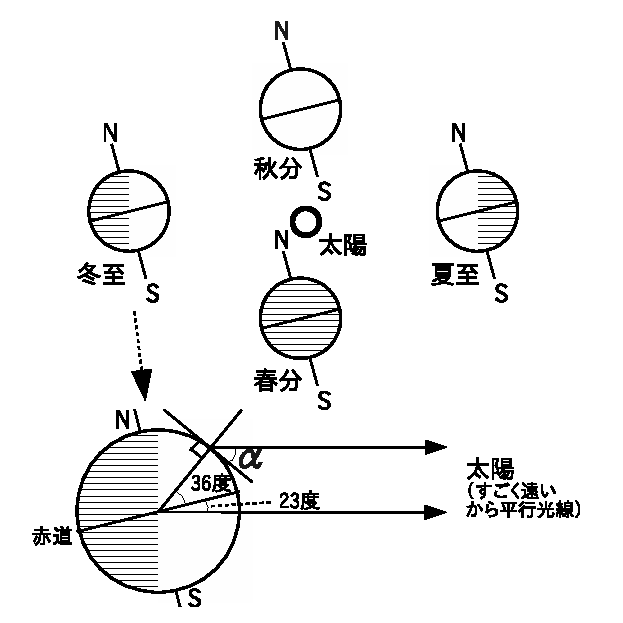
\includegraphics[width=7cm]{sun_angle.eps}
    \caption{問\ref{q:trig_triang_sincos3}の説明図。上: 太陽のまわりをまわる地球。Nは北極, Sは南極。横線で影を
つけたのは, 夜の面。冬至・春分・夏至・秋分は北半球を基準とする(北半球の冬至は南半球の夏至)。
下: 北緯36度での冬至正午の太陽高度$\alpha$の概念図。}\label{fig:sun_angle}
\end{figure}
\begin{enumerate}
\item 春分・秋分\index{しゅんぶん@春分}\index{しゅうぶん@秋分}では$\alpha=54$度になることを示せ。
\item 夏至\index{げし@夏至}では$\alpha=77$度になることを示せ。
\item 冬至\index{とうじ@冬至}では$\alpha=31$度になることを示せ。
\item つくばには, 昔, 高さ220 mの気象観測タワーがあった。太陽南中時に, このタワー
の影はどのくらい長かったか? 春分・秋分, 夏至, 冬至のそれぞれについて答えよ。
\end{enumerate}\end{q}

\noindent{\textbf{答}}\ref{q:trig_triang_sincos3} 小問(1)(2)(3)は中学校の理科で習ったはず。計算には関数電卓を使う。
\begin{enumerate}
\item $\alpha=90-36=54$度
\item $\alpha=90-(36-23)=77$度
\item $\alpha=90-(36+23)=31$度
\item タワーの高さ(220$\,\,$m)を$h$として, $h/\tan\alpha$を求めればよい。有効数字は2桁でよい。\\
春分・秋分: $220\,\text{m}/\tan 54\text{度}\fallingdotseq160$ m。\\
夏至: $220\,\text{m}/\tan 77\text{度}\fallingdotseq51$ m。\\
冬至: $220\,\text{m}/\tan 31\text{度}\fallingdotseq370$ m。
\end{enumerate}
\mv






\section{ベクトルの線型変換}

行列の乗算のルールで, 2次元の列ベクトルに, 左から2次正方行列を掛けると, 結果は, 2次元の列ベクトルになる。例えば, 
\begin{eqnarray}
A=\begin{bmatrix}
1 & 2 \\
0 & 1 \\
\end{bmatrix}
,\,\,\,\, 
{\bf x}=\begin{bmatrix}
2 \\
3 \\
\end{bmatrix}
\end{eqnarray}
とすれば, 
\begin{eqnarray*}
A{\bf x}=\begin{bmatrix}
1 & 2 \\
0 & 1 \\
\end{bmatrix}
\begin{bmatrix}
2 \\
3 \\
\end{bmatrix}
=\begin{bmatrix}
1\times2 + 2\times3 \\
0\times2 + 1\times3 \\
\end{bmatrix}
=\begin{bmatrix}
8 \\
3 \\
\end{bmatrix}
\end{eqnarray*}
となる。このような操作は, 列ベクトルを別の列ベクトルに変換する操作であると
みなすことができる。そこで, このように, 列ベクトルに正方行列を左から
掛けることで別の列ベクトルにする操作のことを, \underline{線型変換} \index{せんけいへんかん@線型変換}
(linear transformation)とか\underline{一次変換} \index{いちじへんかん@一次変換}と呼ぶ
\footnote{大学数学では, 線型変換をもっと一般的・抽象的に定義し直す。}。

さて, 列ベクトルを, 平面上の位置ベクトルとみなせば, 列ベクトルの線型変換は, 
平面上の点を移動させることに相当する。例えば, 
\begin{eqnarray}
A=\begin{bmatrix}
-1 & 0 \\
0 & 1 \\
\end{bmatrix}
\end{eqnarray}
とすれば, 行列$A$による線型変換は, 点$(x, y)$を, 
\begin{eqnarray}
\begin{bmatrix}
-1 & 0 \\
0 & 1 \\
\end{bmatrix}
\begin{bmatrix}
x \\
y \\
\end{bmatrix}
=\begin{bmatrix}
-x \\
y \\
\end{bmatrix}
\end{eqnarray}
というふうに, 点$(-x, y)$に移すことがわかる。これは, $x$座標の正負を逆転
するという操作であり, つまり, $y$軸に関する対称移動である。

\begin{q}\label{q:matrix_lintrans2D0} 以下の行列であらわされる線型変換は, 平面上の点をどのように移すか? 
\begin{edaenumerate}<3>
\item 
\begin{eqnarray*} \begin{bmatrix}
1 & 0 \\
0 & 1 \\
\end{bmatrix}\end{eqnarray*}
\mv
\item 
\begin{eqnarray*} \begin{bmatrix}
1 & 0 \\
0 & -1 \\
\end{bmatrix}\end{eqnarray*}
\mv
\item 
\begin{eqnarray*} \begin{bmatrix}
-1 & 0 \\
0 & -1 \\
\end{bmatrix}\end{eqnarray*}
\mv
\item 
\begin{eqnarray*} \begin{bmatrix}
0 & 1 \\
1 & 0 \\
\end{bmatrix}\end{eqnarray*}
\mv
%\item 
%\begin{eqnarray*} \begin{bmatrix}
%2 & 0 \\
%0 & 2 \\
%\end{bmatrix}\end{eqnarray*}
%\mv
\item 
\begin{eqnarray*} \begin{bmatrix}
2 & 0 \\
0 & 1 \\
\end{bmatrix}\end{eqnarray*}
\mv
\item 
\begin{eqnarray*} \begin{bmatrix}
1 & 0 \\
0 & 0 \\
\end{bmatrix}\end{eqnarray*}
\end{edaenumerate}\end{q}
\mv

\begin{q}\label{q:matrix_lintrans2D2} 前問の, (2), (3), (4)の行列は, いずれも, 2乗したら
単位行列になる。なぜだろうか? 平面上の線型変換という観点から考察せよ。\end{q}
\mv

次に, 平面上の点を回転\index{かいてん@回転}するような変換を考えてみよう。
極座標(\pref{eq:2Dpolar})を考えると, ある点Pの座標(位置ベクトル)は, 
\begin{eqnarray}
\begin{bmatrix}
x \\
y \\
\end{bmatrix}=
\begin{bmatrix}
r \cos \theta \\
r \sin \theta \\
\end{bmatrix}
\end{eqnarray}
と表現できる。ここで$r$は原点OからPまでの距離であり, $\theta$は$x$軸からOPまでの角度(左回り)
である。さて, この点を, 左に$\alpha$だけ回転すると, 当然ながら, その座標は, 
\begin{eqnarray}
\begin{bmatrix}
r \cos (\theta+\alpha) \\
r \sin (\theta+\alpha) \\
\end{bmatrix}
\end{eqnarray}
となる。加法定理(\pref{eq:add_sin1})を使ってこれを変形すれば, 
\begin{eqnarray*}
\begin{bmatrix}
r \cos \theta \cos \alpha - r \sin \theta \sin \alpha\\
r \sin \theta \cos \alpha + r \cos \theta \sin \alpha\\
\end{bmatrix}=
\begin{bmatrix}
x \cos \alpha - y \sin \alpha\\
y \cos \alpha + x \sin \alpha\\
\end{bmatrix}\\
=\begin{bmatrix}
\cos \alpha & -\sin \alpha\\
\sin \alpha & \cos \alpha\\
\end{bmatrix}
\begin{bmatrix}
x\\
y\\
\end{bmatrix}
\end{eqnarray*}
となる。すなわち, 以下の行列:
\begin{eqnarray}
\begin{bmatrix}
\cos \alpha & -\sin \alpha\\
\sin \alpha & \cos \alpha\\
\end{bmatrix}\label{eq:2Drotmatrix}
\end{eqnarray}
が, 「回転という線型変換」を表す行列である。

\begin{faq}{\small\textgt{回転の行列をなかなか覚えられません。どこがcosでどこがsinでどこにマイナスがつくのかとか。}
... \eref{eq:2Drotmatrix}ですね。記憶に自信がないときは, 
試しに$\alpha=0$を代入してみると良いのです。角度0の回転とは,
 何もしないことですから, そのときこの行列は単位行列になるはずです
(実際, そうなるでしょ?)。sinとcosを間違えてたら, 一発でわかります。}\end{faq}

\begin{q}\label{q:matrix_lintrans2D4} 以下のような, 座標平面上の点の移動を表す行列を, それぞれ求めよ:
\begin{enumerate}
\item $x$軸に関して対称移動。
\item 原点に関して対称移動。
\item 原点を中心として, 角$\pi/4$だけ左回りに回転。
\end{enumerate}\end{q}
\mv

\begin{q}\label{q:matrix_lintrans2D6} \eref{eq:2Drotmatrix}の行列を$A$とする。以下を求めよ:\\
(1) $\det A$  (2) $A^{-1}$  (3) $A^2$\end{q}
\vv






\section{固有値と固有ベクトル}
\index{こゆうち@固有値}\index{こゆうべくとる@固有ベクトル}

正方行列$A$に対して, ある実数$\lambda$と, ある(${\bf 0}$でない)ベクトル${\bf x}$によって, 
\begin{eqnarray}
A{\bf x}=\lambda {\bf x}\label{eq:def_eigenvec}
\end{eqnarray}
となるとき, ${\bf x}$を$A$の\underline{固有ベクトル} (eigenvector)といい, 
$\lambda$を$A$の\underline{固有値} (eigenvalue)という(定義)。
これは, 行列の応用において, 非常に重要な概念である。\\

{\small 注: なぜか\eref{eq:def_eigenvec}を${\bf x}A={\bf x}\lambda$のように
書く人がいる。特殊な状況設定をすればこのように書くことも
無いではないのだが(それを今の段階で説明すると君は絶対に混乱する), 
そんなややこしいことをしないで, 素直に\eref{eq:def_eigenvec}の形で
覚えて欲しい。数と数の積ならどちらを先に書いてもかまわないのだが, 
行列やベクトルがからむ「積」は, 書き方や順序を不用意に
変えてはならないのだ。}

\begin{faq}{\small\textgt{固有ベクトルの定義で, なぜ${\bf x}$が${\bf 0}$でないという条件が
ついているのですか?}
... もし${\bf x}={\bf 0}$だと, $A$がどんな正方行列であろうが, また, $\lambda$
がどんなスカラーであろうが, $A{\bf x}=\lambda{\bf x}$が成り立っちゃうから
です。そういう「当たり前」の場合を, 固有ベクトルとはみなさない約束なのです。}\end{faq}

\begin{exmpl}\label{ex:matrix_eigen1} 以下の行列の固有値と固有ベクトルを求めてみよう:
\begin{eqnarray}
A=\begin{bmatrix}
5 & 3 \\
4 & 1 \\
\end{bmatrix}
\end{eqnarray}
固有値を$\lambda$, 固有ベクトルを${\bf x}$とすると, 定義から, $A{\bf x}=\lambda {\bf x}$が成り立つ。つまり, 
\begin{eqnarray}
A{\bf x}-\lambda {\bf x}={\bf 0}
\end{eqnarray}
である。ここで, $\lambda {\bf x}=\lambda E {\bf x}$と考えれば, 上の式は, 
\begin{eqnarray}
A{\bf x}-\lambda E{\bf x}={\bf 0}
\end{eqnarray}
すなわち, 
\begin{eqnarray}
(A-\lambda E){\bf x}={\bf 0}\label{eq:matrix_eigen_eq0}
\end{eqnarray}
となる。すなわち, 
\begin{eqnarray}
(A-\lambda E){\bf x}=
\begin{bmatrix}
5-\lambda & 3 \\
4          & 1-\lambda \\
\end{bmatrix}
\begin{bmatrix}
x \\
y \\
\end{bmatrix}
=\begin{bmatrix}
0 \\
0 \\
\end{bmatrix}\label{eq:matrix_eigen_eq000}
\end{eqnarray}
となる。さて, もしこの係数行列$A-\lambda E$に逆行列が存在すると仮定すれば, 
上の式の両辺に左から$(A-\lambda E)^{-1}$をかけて, 
\begin{eqnarray}
{\bf x}
=(A-\lambda E)^{-1}
\begin{bmatrix}
0 \\
0 \\
\end{bmatrix}
\end{eqnarray}
となる。$(A-\lambda E)^{-1}$がどんな行列であれ, この右辺は零ベクトル
になるしかない。すなわち, 
\begin{eqnarray}
{\bf x}
=\begin{bmatrix}
0 \\
0 \\
\end{bmatrix}={\bf 0}
\end{eqnarray}
となってしまう。これは, 固有ベクトルの定義に反している。従って, 
係数行列$A-\lambda E$に逆行列が存在してはならない\footnote{この論理は背理法である。}。従って, その行列式
は0にならねばならない。すなわち, 
\begin{eqnarray}
\det(A-\lambda E)=0\label{eq:matrix_tokusei}
\end{eqnarray}
である。\eref{eq:matrix_tokusei}を行列$A$の\underline{特性方程式} \index{とくせいほうていしき@特性方程式}
という(固有方程式ともいう\index{こゆうほうていしき@固有方程式})。これを解くと, 
\begin{eqnarray*}
&&(5-\lambda)(1-\lambda)-3\times4\\
&&=\lambda^2-6\lambda-7=(\lambda+1)(\lambda-7)=0
\end{eqnarray*}
となり, $\lambda=-1$と, $\lambda=7$となる。これで固有値が求まった。

では固有ベクトルを求めよう。まず, $\lambda=-1$のとき, 上の連立一次方程式(\ref{eq:matrix_eigen_eq000})は, 
\begin{eqnarray}
(A-\lambda E){\bf x}=
\begin{bmatrix}
6          & 3 \\
4          & 2 \\
\end{bmatrix}
\begin{bmatrix}
x \\
y \\
\end{bmatrix}
=\begin{bmatrix}
0 \\
0 \\
\end{bmatrix}\end{eqnarray}
となる。明らかに, この方程式は不定であり, これを満たす解は無数にあるが, 代表的に, 
\begin{eqnarray}
\begin{bmatrix}
x \\
y \\
\end{bmatrix}
=\begin{bmatrix}
1 \\
-2 \\
\end{bmatrix}
\end{eqnarray}
としよう。これが, 固有ベクトルのひとつである。

次に, $\lambda=7$のとき, 連立一次方程式(\ref{eq:matrix_eigen_eq0})は, 
\begin{eqnarray}
(A-\lambda E){\bf x}=
\begin{bmatrix}
-2         & 3 \\
4          & -6 \\
\end{bmatrix}
\begin{bmatrix}
x \\
y \\
\end{bmatrix}
=\begin{bmatrix}
0 \\
0 \\
\end{bmatrix}\end{eqnarray}
となる。この方程式も不定であり, これを満たす解は無数にあるが, 代表的に, 
\begin{eqnarray}
\begin{bmatrix}
x \\
y \\
\end{bmatrix}
=\begin{bmatrix}
3 \\
2 \\
\end{bmatrix}
\end{eqnarray}
としよう。これも, 固有ベクトルのひとつである。以上より, 行列$A$について, 
\begin{eqnarray*}\begin{cases}
\text{固有値が}-1\text{のとき, 固有ベクトル}
\begin{bmatrix}
1 \\
-2 \\
\end{bmatrix}\\
\\
\text{固有値が}7\text{のとき, 固有ベクトル}
\begin{bmatrix}
3 \\
2 \\
\end{bmatrix}
\end{cases}\end{eqnarray*}
である。
(例おわり)\end{exmpl}

このように, 固有値と固有ベクトルは, 互いに対になっている。一般に, 固有値・固有ベクトルの対
は, 高々, その行列の次数の数だけ存在する(中にはそれに足りない行列もあるが)。

\begin{q}\label{q:matrix_eigen2D0} 以下の行列について, 固有値と固有ベクトルを求めよ。
\begin{eqnarray} \begin{bmatrix}
2 & 1\\
2 & 3\\
\end{bmatrix}\label{eq:matrix_lintrans_mondai}\end{eqnarray}
\end{q}\mv


\begin{figure}[ht]
    \centering
    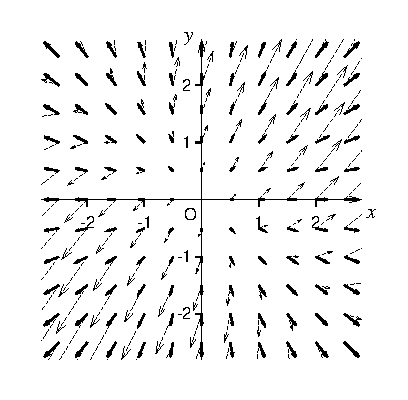
\includegraphics[width=8cm]{eigen.eps}
    \caption{\eref{eq:matrix_lintrans_mondai}の行列による線型変換のイメージ。
各点$(x, y)$にはベクトル$(x, y)$と(実線矢印), それを\eref{eq:matrix_lintrans_mondai}の行列
で線型変換したベクトル(点線矢印)が描かれている。2つの矢印が同方向に向いているとき(重なっているとき)
が固有ベクトルである。特に, 固有値が1のときの固有ベクトルは, もとの
ベクトルと, 向きも大きさも同じであることに注意しよう。}
\end{figure}
\mv

固有値や固有ベクトルが(実数の範囲では)求まらないような行列もある。例えば, \peref{eq:2Drotmatrix}
で$\alpha=\pi/3$とする。すなわち, 
\begin{eqnarray}
\begin{bmatrix}
\cos (\pi/3) & -\sin (\pi/3)\\
\sin (\pi/3) & \cos (\pi/3)\\
\end{bmatrix}
=\begin{bmatrix}
1/2 & -\sqrt{3}/2\\
\sqrt{3}/2 & 1/2\\
\end{bmatrix}\nonumber\\
\label{eq:matrix_lintrans_rot_pi_3}
\end{eqnarray}
を考える。これは, 原点を中心として角$\pi/3$だけ左回りに回転するような変換を表す行列である。

\begin{q}\label{q:matrix_eigen2D2} \eref{eq:matrix_lintrans_rot_pi_3}の行列について, 
\begin{enumerate}
\item 特性方程式は次式のようになることを示せ:
\begin{eqnarray}\lambda^2-\lambda+1=0\end{eqnarray}
\item この特性方程式は実数解を持たないことを示せ。
\end{enumerate}\end{q}
\mv


このように, \eref{eq:matrix_lintrans_rot_pi_3}の行列は実数の範囲で固有値や
固有ベクトルを持たない。つまり, この行列による線型変換では, 向きを変えないベクトルが
存在しない(全てのベクトルは向きを変える), ということになる。そもそも
この変換は原点を中心として全てのベクトルを左回りに回転させるのだから, 当然である。

\begin{figure}[ht]
    \centering
    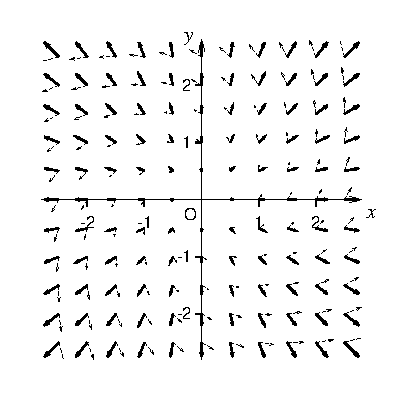
\includegraphics[width=8cm]{rot_vectf.eps}
    \caption{\eref{eq:matrix_lintrans_rot_pi_3}の行列による線型変換のイメージ。
各点$(x, y)$にはベクトル$(x, y)$と(実線矢印), それを\eref{eq:matrix_lintrans_rot_pi_3}
の行列で線型変換したベクトル(点線矢印)が描かれている。
もとのベクトルは全て, 左回りに回転したベクトルに移るので, 「向きを変えないベクトル」
(つまり固有ベクトル)が存在しない。}
\end{figure}
\vv



\section{対角化}

先の例\ref{ex:matrix_eigen1}(P.\pageref{ex:matrix_eigen1})で, 
\begin{eqnarray}
A=\begin{bmatrix}
5 & 3 \\
4 & 1 \\
\end{bmatrix}
\end{eqnarray}
という行列$A$について, 
\begin{eqnarray*}\begin{cases}
\text{固有値が}-1\text{のとき, 固有ベクトル}
\begin{bmatrix}
1 \\
-2 \\
\end{bmatrix}\\
\\
\text{固有値が}7\text{のとき, 固有ベクトル}
\begin{bmatrix}
3 \\
2 \\
\end{bmatrix}
\end{cases}\end{eqnarray*}
であることが示された。すなわち, 
\begin{eqnarray}\begin{cases}
\begin{bmatrix}
5 & 3 \\
4 & 1 \\
\end{bmatrix}
\begin{bmatrix}
1 \\
-2 \\
\end{bmatrix}
=-1\times\begin{bmatrix}
1 \\
-2 \\
\end{bmatrix}\\
\\
\begin{bmatrix}
5 & 3 \\
4 & 1 \\
\end{bmatrix}
\begin{bmatrix}
3 \\
2 \\
\end{bmatrix}
=7\times\begin{bmatrix}
3 \\
2 \\
\end{bmatrix}
\end{cases}\end{eqnarray}
である。これらをひとまとめにすると, 
\begin{eqnarray*}
\begin{bmatrix}
5 & 3 \\
4 & 1 \\
\end{bmatrix}
\begin{bmatrix}
1 & 3\\
-2 & 2\\
\end{bmatrix}
=\begin{bmatrix}
1 & 3\\
-2 & 2\\
\end{bmatrix}
\begin{bmatrix}
-1 & 0 \\
0 & 7 \\
\end{bmatrix}
\end{eqnarray*}
とできる\footnote{固有ベクトルの並べ順を左右入れ替えて, 
\begin{eqnarray*}
\begin{bmatrix}
5 & 3 \\
4 & 1 \\
\end{bmatrix}
\begin{bmatrix}
3 & 1\\
2 & -2\\
\end{bmatrix}
=\begin{bmatrix}
3 & 1\\
2 & -2\\
\end{bmatrix}
\begin{bmatrix}
7 & 0 \\
0 & -1 \\
\end{bmatrix}
\end{eqnarray*}
としてもよい。その場合, \eref{eq:matrix_orthogonalize_9}に相当する式は, 
\begin{eqnarray*}
Q=\begin{bmatrix}
3 & 1\\
2 & -2\\
\end{bmatrix}
\text{として, }\,\,\,
Q^{-1}AQ
=\begin{bmatrix}
7 & 0 \\
0 & -1 \\
\end{bmatrix}
\end{eqnarray*}
}。すると, 
\begin{eqnarray}
\begin{bmatrix}
1 & 3\\
-2 & 2\\
\end{bmatrix}^{-1}
\begin{bmatrix}
5 & 3 \\
4 & 1 \\
\end{bmatrix}
\begin{bmatrix}
1 & 3\\
-2 & 2\\
\end{bmatrix}
=\begin{bmatrix}
-1 & 0 \\
0 & 7 \\
\end{bmatrix}\label{eq:matrix_orthogonalize_6}
\end{eqnarray}
となることがわかる。ここで, 2つの固有ベクトルを列ベクトルとして並べてできる行列を$P$とする。つまり, 
\begin{eqnarray}
P=\begin{bmatrix}
1 & 3\\
-2 & 2\\
\end{bmatrix}
\end{eqnarray}
とすると, \eref{eq:matrix_orthogonalize_6}は, 
\begin{eqnarray}
P^{-1}AP
=\begin{bmatrix}
-1 & 0 \\
0 & 7 \\
\end{bmatrix}\label{eq:matrix_orthogonalize_9}
\end{eqnarray}
である。このように, 与えられた行列(ここでは$A$)に対して, ある行列$P$によって, $P^{-1}AP$
とすることで, 非対角成分が0の行列(そのような行列を対角行列\index{たいかくぎょうれつ@対角行列}という)
にすることを, \underline{対角化}\index{たいかくか@対角化}という。上の説明でわかるように, 
ある行列$A$を対角化するには, 次のような手順をとる:
\begin{itemize}
\item $A$の特性方程式を立てる。
\item それを解いて, $A$の固有値を求める。
\item 各固有値に対応する固有ベクトルを求める。
\item $A$の固有ベクトルを列ベクトルとして並べてできる行列を$P$とおく(慣習的には, 固有値の大きい順に)。
\item すると, $P^{-1}AP$は対角行列になる。その対角行列の対角成分(行番号と列番号が同じ成分)には, $A$の固有値が並ぶ。
\end{itemize}
\mv

\begin{q}\label{q:matrix_orth2D0} 以下の行列を対角化せよ:
\begin{eqnarray} \begin{bmatrix}
-1 & 2\\
-6 & 6\\
\end{bmatrix}\end{eqnarray}
\end{q}\mv

さて, ある2次正方行列$A$が, 行列$P$によって対角化されるとき, 
\begin{eqnarray}
P^{-1}AP
=\begin{bmatrix}
\lambda_1 & 0 \\
0 & \lambda_2 \\
\end{bmatrix}
\end{eqnarray}
となる($\lambda_1$と$\lambda_2$は$A$の固有値である)。両辺に, 左から$P$を, 右から$P^{-1}$を
それぞれ掛けると, 
\begin{eqnarray}
A
=P\begin{bmatrix}
\lambda_1 & 0 \\
0 & \lambda_2 \\
\end{bmatrix}P^{-1}
\end{eqnarray}
となる。従って, $A$の行列式は, 
\begin{eqnarray}
&&\det A\nonumber\\
&&=\det\Bigl(P\begin{bmatrix}
\lambda_1 & 0 \\
0 & \lambda_2 \\
\end{bmatrix}P^{-1}\Bigr)
=\det P\det\begin{bmatrix}
\lambda_1 & 0 \\
0 & \lambda_2 \\
\end{bmatrix}\det P^{-1}\nonumber\\
&&=\det P\det P^{-1}\det\begin{bmatrix}
\lambda_1 & 0 \\
0 & \lambda_2 \\
\end{bmatrix}=\det\begin{bmatrix}
\lambda_1 & 0 \\
0 & \lambda_2 \\
\end{bmatrix}\nonumber\\
&&=\lambda_1\lambda_2
\end{eqnarray}
となる(ここで\eref{eq:detABdetAdetB}, \eref{q:matrix_det_inv}を使った)。
つまり, 行列式は, 固有値の積に等しい (定理)。
\hv





\section{特殊な行列}

行列$A$の行と列を入れ替えてできる行列を, 
行列$A$の\underline{転置行列} \index{てんちぎょうれつ@転置行列}と呼び, $^\text{t}A$
とあらわす。すなわち, $A=(a_{ij})$とするとき, $^\text{t}A=(b_{ij})$は, $b_{ij}=a_{ji}$を
満たすような行列である(定義)。

\begin{exmpl} \peref{eq:matrix32ex}の行列$A$の転置行列は, 
\begin{eqnarray}
^\text{t}A=\begin{bmatrix}
1 & -1\\
2 & 1\\
3 & 0\\
\end{bmatrix}
\label{eq:matrix32ex_trans}
\end{eqnarray}
である(例おわり)\end{exmpl}

一般に$n\times m$行の転置行列は$m\times n$行列になることは明らかだろう。特に, 
正方行列は行数と列数が互いに等しいから, 転置行列も正方行列になる。

正方行列$A$が, $^\text{t}A=A$を満たすとき, $A$を\underline{対称行列} (symmetric matrix)
\index{たいしょうぎょうれつ@対称行列}という(定義)。例えば, 以下の行列$B$は対称行列である:
\begin{eqnarray}
B=\begin{bmatrix}
1  & -1 & 3\\
-1 & 2  & 0\\
3  & 0  & 4\\
\end{bmatrix}
\label{eq:matrix_symmetric}\end{eqnarray}
単位行列は対称行列である。

正方行列$A$が, $^\text{t}A=A^{-1}$を満たすとき, $A$を\underline{直交行列} (orthogonal matrix)
という\index{ちょっこうぎょうれつ@直交行列} (定義)。例えば, \eref{eq:2Drotmatrix}は
直交行列である(確認せよ)。単位行列は直交行列でもある(確認せよ)。

\begin{q}\label{q:matrix_symm_orth2D} \pref{q:matrix_lintrans2D0}の
問\ref{q:matrix_lintrans2D0}の行列の中から, 対称行列と直交行列をそれぞれ選び出せ。\end{q}
\hv


%\begin{q}\label{q:matrix_English} 以下の言葉を英訳せよ:
%\begin{edaenumerate}<3>
%\item 単位行列
%\item 逆行列
%\item 行列式
%\item 線型変換
%\item 固有値
%\end{edaenumerate}
%\end{q}\mv


\noindent{\textbf{答}}\ref{q:matrix_lintrans2D0}  
\begin{enumerate}
\item 同じ点に移動(というか, そもそも, 移動させない)。
\item $x$軸に関して対称な点に移動。
\item 原点に関して対称な点に移動。 
\item 直線$y=x$に関して対称な点に移動。
%\item $x$方向も$y$方向も2倍に拡大。
\item $x$方向だけを2倍に拡大。
\item $x$軸に下ろした垂線の足に移動。(射影)
\end{enumerate}
\mv

%
\noindent{\textbf{答}}\ref{q:matrix_lintrans2D2}  (2), (3), (4)は, いずれも, 線または点に関する対称変換なので, 
2回繰り返すともとに戻る。従って, それらをあらわす行列を2乗したもの
は単位行列になる。
\mv

%
\noindent{\textbf{答}}\ref{q:matrix_lintrans2D4}  
\begin{edaenumerate}<3>
\item \begin{eqnarray*}\begin{bmatrix}
1 & 0 \\
0 & -1 \\\end{bmatrix}\end{eqnarray*}
\item \begin{eqnarray*}\begin{bmatrix}
-1 & 0 \\
0 & -1 \\
\end{bmatrix}\end{eqnarray*}
\item \begin{eqnarray*}\begin{bmatrix}
\frac{1}{\sqrt{2}} & -\frac{1}{\sqrt{2}} \\
\frac{1}{\sqrt{2}} & \frac{1}{\sqrt{2}} \\
\end{bmatrix}\end{eqnarray*}
\end{edaenumerate}
\mv

\noindent{\textbf{答}}\ref{q:matrix_lintrans2D6} 
\begin{enumerate}
\item $\,\,\,\,\det A=\cos^2\alpha+\sin^2\alpha=1$
\item \begin{eqnarray}
\begin{bmatrix}
\cos\alpha & \sin\alpha \\
-\sin\alpha & \cos\alpha \\\end{bmatrix}
\end{eqnarray}
注:これは, 角$(-\alpha)$の回転をあらわす行列である。
\item (計算過程は省略)
\begin{eqnarray}\begin{bmatrix}
\cos2\alpha & -\sin2\alpha \\
\sin2\alpha & \cos2\alpha \\\end{bmatrix}
\end{eqnarray}
注:これは, 角$2\alpha$の回転をあらわす行列である。
\end{enumerate}
\mv



% 固有値と固有ベクトル
% 
\noindent{\textbf{答}}\ref{q:matrix_eigen2D0}  この行列を$A$とすると, 
その特性方程式は, \eref{eq:matrix_tokusei}より, 
\begin{eqnarray*}
&&\det(A-\lambda E)=(2-\lambda)(3-\lambda)-1\times2\\
&&=\lambda^2-5\lambda+4=(\lambda-1)(\lambda-4)=0
\end{eqnarray*}
となる。これを満たすのは, $\lambda=1$と, $\lambda=4$である。
これが固有値である。では固有ベクトルを求めよう。まず, $\lambda=1$のとき, 
\begin{eqnarray}
(A-\lambda E){\bf x}=
\begin{bmatrix}
1          & 1 \\
2          & 2 \\
\end{bmatrix}
\begin{bmatrix}
x \\
y \\
\end{bmatrix}
=\begin{bmatrix}
0 \\
0 \\
\end{bmatrix}\end{eqnarray}
となる。これを満たす解は無数にあるが, 代表的に, 
\begin{eqnarray}
\begin{bmatrix}
x \\
y \\
\end{bmatrix}
=\begin{bmatrix}
1 \\
-1 \\
\end{bmatrix}
\end{eqnarray}
としよう。これが, 固有ベクトルのひとつである。

次に, $\lambda=4$のとき, 
\begin{eqnarray}
(A-\lambda E){\bf x}=
\begin{bmatrix}
-2         & 1 \\
2          & -1 \\
\end{bmatrix}
\begin{bmatrix}
x \\
y \\
\end{bmatrix}
=\begin{bmatrix}
0 \\
0 \\
\end{bmatrix}\end{eqnarray}
となる。これを満たす解も無数にあるが, 代表的に, 
\begin{eqnarray}
\begin{bmatrix}
x \\
y \\
\end{bmatrix}
=\begin{bmatrix}
1 \\
2 \\
\end{bmatrix}
\end{eqnarray}
としよう。これも, 固有ベクトルのひとつである。以上より, 行列$A$について, 
\begin{eqnarray*}\begin{cases}
\text{固有値が}1\text{のとき, 固有ベクトル}
\begin{bmatrix}
1 \\
-1 \\
\end{bmatrix}\\
\\
\text{固有値が}4\text{のとき, 固有ベクトル}
\begin{bmatrix}
1 \\
2 \\
\end{bmatrix}
\end{cases}\end{eqnarray*}
である\footnote{ただし, 固有ベクトルはこれらを何倍かしたもの(0倍以外)でもかまわない。}。
\mv

% 
%2011.0906 ヤマサキ解答追加。
\noindent{\textbf{答}}\ref{q:matrix_eigen2D2} 
\begin{enumerate}
\item \eref{eq:matrix_lintrans_rot_pi_3}の行列を$A$と置くと, $A$の特性方程式は, 
\begin{eqnarray*}
\text{det}(A-\lambda E)=
\text{det}
\begin{bmatrix}
\frac{1}{2}-\lambda & -\frac{\sqrt{3}}{2} \\
\frac{\sqrt{3}}{2} & \frac{1}{2}-\lambda \\
\end{bmatrix}\\
=\bigl(\frac{1}{2} - \lambda\bigr)^2 + \frac{3}{4}=\lambda^2 -\lambda +1=0
\end{eqnarray*}
\item この特性方程式は2次方程式である。2次方程式が実数解を持つかどうかは, 2次方程式の判別式(\peref{eq:Q(uadratic)_E(quations)_D(iscriminant)})を調べればわかる。ここで, この特性方程式の判別式$D$は, 
\begin{eqnarray*}
D = (-1)^2 -4 \cdot 1 \cdot 1 = -3 < 0
\end{eqnarray*}
したがって, この特性方程式は実数解を持たない。
\end{enumerate}
\mv

%
\noindent{\textbf{答}}\ref{q:matrix_orth2D0} (略解: 本来は固有値と固有ベクトルを求める過程も書くこと。)
\begin{eqnarray}
\begin{bmatrix}
2 & 1\\
3 & 2\\
\end{bmatrix}^{-1}
\begin{bmatrix}
-1 & 2 \\
-6 & 6 \\
\end{bmatrix}
\begin{bmatrix}
2 & 1\\
3 & 2\\
\end{bmatrix}
=\begin{bmatrix}
2 & 0 \\
0 & 3 \\
\end{bmatrix}
\end{eqnarray}
または, 以下のようにしてもよい:
\begin{eqnarray}
\begin{bmatrix}
1 & 2\\
2 & 3\\
\end{bmatrix}^{-1}
\begin{bmatrix}
-1 & 2 \\
-6 & 6 \\
\end{bmatrix}
\begin{bmatrix}
1 & 2\\
2 & 3\\
\end{bmatrix}
=\begin{bmatrix}
3 & 0 \\
0 & 2 \\
\end{bmatrix}
\end{eqnarray}
\mv

%
\noindent{\textbf{答}}\ref{q:matrix_symm_orth2D}\\
対称行列: 全て。直交行列: (1), (2), (3), (4)\\


%
\noindent{\textbf{答}}\ref{q:mtrix_exm_mMrkov}
\begin{enumerate}
\item (略解) $\lambda$を固有値とすると, $A$の特性方程式は
\begin{equation*}
\lambda^2-1.7\lambda+0.7=(\lambda-1)(\lambda-0.7)=0
\end{equation*}
となり, $\lambda=1, 0.7$。それぞれに対応する固有ベクトルは, 代表的に, 
\begin{equation*}
\begin{bmatrix}
1\\
2
\end{bmatrix},\,\,\,\,\,
\begin{bmatrix}
1\\
-1\\
\end{bmatrix}
\end{equation*}
である。これを並べた行列を$P$とすると, 
\begin{equation}
P=\begin{bmatrix}
1 & 1\\
2 & -1\\
\end{bmatrix}
\end{equation}
これによって, 
\begin{equation}
P^{-1}AP=\begin{bmatrix}
1 & 0\\
0 & 0.7\\
\end{bmatrix}
\end{equation}
\item 略。
\item
\begin{eqnarray*}
(P^{-1}AP)^n&=&(P^{-1}AP)(P^{-1}AP)\cdots(P^{-1}AP)\\
&=&P^{-1}APP^{-1}AP\cdots P^{-1}AP\\
&=&P^{-1}AA\cdots AP\\
&=&P^{-1}A^nP
\end{eqnarray*}
となる。一方, 前小問より, 
\begin{equation}
(P^{-1}AP)^n=\begin{bmatrix}
1 & 0\\
0 & 0.7\\
\end{bmatrix}^n
=\begin{bmatrix}
1 & 0\\
0 & 0.7^n\\
\end{bmatrix}
\end{equation}
従って, 
\begin{equation}
P^{-1}A^nP
=\begin{bmatrix}
1 & 0\\
0 & 0.7^n\\
\end{bmatrix}
\end{equation}
従って, 
\begin{eqnarray*}
A^n
&=&P\begin{bmatrix}
1 & 0\\
0 & 0.7^n\\
\end{bmatrix}P^{-1}\\
&=&\cdots=\frac{1}{3}\begin{bmatrix}
1+2\times0.7^n & 1-0.7^n\\
2-2\times0.7^n & 2+0.7^n\\
\end{bmatrix}
\end{eqnarray*}
\item $n=3$とすると, \\
\begin{eqnarray*}
&&\begin{bmatrix}
b_3\\
f_3\\
\end{bmatrix}
=A^3\begin{bmatrix}
b_0\\
f_0\\
\end{bmatrix}
=\begin{bmatrix}
0.562 & 0.219\\
0.438 & 0.781\\
\end{bmatrix}
\begin{bmatrix}
80\\
20\\
\end{bmatrix}
=\begin{bmatrix}
49.34\\
50.66\\
\end{bmatrix}
\end{eqnarray*}
\\である。従って, 裸地と森林がほぼ同面積(50$\,\,$km$^2$程度)になると予想される。
\item (3)の答えで$n\rightarrow\infty$とすると, $A^n$は
\begin{equation}
\begin{bmatrix}
1/3 & 1/3\\
2/3 & 2/3\\
\end{bmatrix}
\end{equation}
に収束する。従って, \\
\begin{eqnarray*}
\begin{bmatrix}
b_n\\
f_n\\
\end{bmatrix}
&\rightarrow&
\begin{bmatrix}
1/3 & 1/3\\
2/3 & 2/3\\
\end{bmatrix}
\begin{bmatrix}
80\\
20\\
\end{bmatrix}
=\begin{bmatrix}
100/3\\
200/3\\
\end{bmatrix}
\fallingdotseq\begin{bmatrix}
33\\
67\\
\end{bmatrix}
\end{eqnarray*}
\\従って, 裸地33$\,\,$km$^2$, 森林67$\,\,$km$^2$と予想される。
\end{enumerate}


